
%\begin{document}

\chapter{Pixelated Reconstruction of Gravitational Lenses using Recurrent Inference Machine}\label{chap:censai}
\thispagestyle{empty}

\begin{center}
Alexandre Adam,$^{1,2}$
Laurence Perreault-Levasseur,$^{1,2,3}$
Yashar Hevazeh$^{1,3}$
\end{center}

\vspace*{0.5cm}
\noindent $^{1}$\textit{D\'{e}partement de physique, Universit\'{e} de Montr\'{e}al, Montr\'{e}al, H3C 3J7, Canada}\\
$^{2}$\textit{Mila - Quebec Artificial Intelligence Institute, Montréal, Canada}\\
$^{3}$\textit{Center for Computational Astrophysics, Flatiron Institute, 162 5th Avenue, 10010, New York, NY, USA}\\
\vspace*{1.5cm}

\begin{center}
Un résumé de cet article à été accepté à l'atelier \textit{Machine Learning for Astrophysics
Workshop at the Thirty-ninth International Conference on Machine Learning (ICML 2022)}. \\
Cet article sera soumis à la revue \textit{The Astrophysical Journal} (ApJ) durant le prochains mois. 
\end{center}


\clearpage
%\begin{resume}
\section*{Résumé}
Modéliser les lentilles gravitationnelles dans le but de quantifier les distorsions des images 
d'arrière-plan et de reconstruire la densité de masse de la lentille en avant-plan est encore aujourd'hui 
un problème difficile, posant un défi computationnel majeur. Avec le nombre croissant de lentilles découvertes et 
la résolution croissante des images de ces systèmes, la tâche d'exploiter complètement l'information qu'elles contiennent 
est présentement un problème hors d'atteinte pour les algorithmes traditionnels.
Dans ce travail, on introduit un réseau neuronal récurrent basé sur les machines à inférence récurentielles (RIM) 
pour reconstruire simultanément une image non déformée de la source en arrière-plan et une image de la densité de masse de la lentille. 
La méthode que nous présentons reconstruit de façon itérative les paramètres du modèle (les pixels de la source et de la densité de la lentille) 
en apprenant le processus d'optimisation de la vraisemblance étant donné une observation et un modèle physique (une simulation des chemins lumineux), 
régularisée par des biais inductifs appris implicitement par le réseau de neurones avec les données d'entraînement. 
Comparée aux méthodes traditionnelles basées sur des modèles paramétriques de la densité de masse, notre approche 
est significativement plus expressive et peut reconstruire des distributions de masses complexes, ce qu'on démontre 
en utilisant des galaxies lentilles réalistes provenant de la simulation cosmologique hydrodynamique IllustrisTNG.

\textbf{Mots-clés:} Lentilles gravitationnelles ---
        Simulations astrophysiques  ---
        Inférence non-paramétrique ---
        Réseaux neuronaux convolutifs.
%\end{resume}


\section*{Abstract}
Modeling strong gravitational lenses in order to 
quantify the distortions in the images of background sources and 
to reconstruct the mass density in the foreground lenses has 
traditionally been a difficult computational challenge. 
As the quality of gravitational lens images increases, the task of fully exploiting the information they contain 
becomes computationally and algorithmically more difficult. 
In this work, we use a neural network based on the Recurrent Inference Machine (RIM) to simultaneously reconstruct 
an undistorted image of the background source and the lens mass density distribution as pixelated maps. 
The method we present iteratively reconstructs the model parameters (the source and density map pixels) by learning 
the process of optimization of their likelihood given the data using the physical model (a ray-tracing simulation), regularized
by a prior implicitly learned by the neural network through its training data. When compared to more traditional parametric models, 
the proposed method is significantly more expressive and can reconstruct complex mass distributions, 
which we demonstrate by using realistic lensing galaxies taken from the cosmological hydrodynamic simulation IllustrisTNG. 

\textbf{Keywords:} Gravitational lensing (670) ---
        Astronomical simulations (1857) ---
        Nonparametric inference (1903) ---
        Convolutional Neural Networks (1938).


%\author{\href{https://orcid.org/0000-0001-8806-7936}{
\includegraphics[width=8pt]{orcid.pdf}} Alexandre Adam }
%\affiliation{Department of Physics, Université de Montréal, Montréal, Canada}
%\affiliation{Mila - Quebec Artificial Intelligence Institute, Montréal, Canada}

%\author{\href{https://orcid.org/0000-0003-3544-3939}{
\includegraphics[width=8pt]{orcid.pdf}} Laurence Perreault-Levasseur }
%\affiliation{Department of Physics, Université de Montréal, Montréal, Canada}
%\affiliation{Mila - Quebec Artificial Intelligence Institute, Montréal, Canada}
%\affiliation{Center for Computational Astrophysics, Flatiron Institute, 162 5th Avenue, 10010, New York, NY, USA}


%\author{ \href{https://orcid.org/0000-0002-8669-5733}{
\includegraphics[width=8pt]{orcid.pdf}} Yashar Hezaveh}
%\affiliation{Department of Physics, Université de Montréal, Montréal, Canada}
%\affiliation{Center for Computational Astrophysics, Flatiron Institute, 162 5th Avenue, 10010, New York, NY, USA}

%\begin{resume}
        
%\end{resume}



%\keywords{
        %Gravitational lensing (670) ---
        %Astronomical simulations (1857) ---
        %Nonparametric inference (1903) ---
        %Convolutional Neural Networks (1938)
%}

%\tableofcontents



\section{Introduction}

%A gravitational lens is composed of 
%massive objects ---or \textit{deflectors}--- in the line of sight that 
%magnify and distort luminous
%background objects like early-type star-forming galaxies \citep{Viera2013,Marrone2018,Rizzo2020,Sun2021},
%otherwise too faint to study with our 
%current ground and orbital telescope facilities. 
%This distortion is a very good tracer of mass, 
%independent of the electromagnetic 
%signature of the foreground deflector. As such, it 
%is one of the rare ways to study the 
%properties of dark matter 
%halos via its spatial distribution at the very small scales 
%\citep{Dala2002,Treu2004,Hezaveh2016,Gilman2020,Gilman2021}. 
%Gravitational lenses also act as cosmological rulers against which we can measure the 
%expansion rate of the universe by monitoring the flickering light of multiply imaged quasars 
%\citep[and reference therein]{Treu2016td,Millon2020} 
%or the dimming of multiply imaged supernovae \citep{Refsdal1964,Treu2016refsdal,Grillo2018}. 
%A central component of such cosmographic analysis is the 
%careful mass modelling of the lensing galaxy \citep{Chen2019,Wong2020} or 
%lensing galaxy clusters \citep{Kneib2011,Hoekstra2013,Natarajan2017,Bergamini2018,Jauzac2021}. 


%A common practice in galaxy mass modelling is to assume that the mass distribution of the 
%main deflector follows a power law $\rho \propto r^{-\gamma'}$ \citep{Keeton2001}.
%Following spectroscopic measurement 
%of the velocity dispersion of early-type galaxies, 
%a singular isothermal profile $\gamma' = 2$ can provide a good starting point for analysis
%\citep{Koopman2006,Barnabe2009,Auger2010}. For cosmographic measurments, 
%this assumption is relaxed by leaving the slope of the profile as 
%a free parameter in the mass modelling stage 
%since the isothermal approximation will induce a bias in the measurement 
%of the Hubble constant \citep{Treu2004,Birrer2020}. 
%Composite models can also be constructed as in \citet{Millon2020}, who 
%uses a Navarro-Frenk-White profile 
%\citep{Navarro1997} to model the dark matter halo that host the lensing galaxy 
%and a Sérsic profile \citep{Sersic1963} 
%to model the baryonic component of the galaxy. Even though these models 
%could produce a large range of profiles, best fit models often 
%have an average slope akin to an isothermal profile. This 
%observation is dubbed the \textit{bulge-halo conspiracy} \citep{Dutton2014}.

%Detailed modelling of high resolution images with high 
%signal-to-noise ratio (SNR) will additionally require external perturbations 
%to the main lensing galaxy coming from its local environment 
%\citep{Sluse2017,Wong2017,Birrer2019,Rusu2019} and 
%from the line of sight \citep{Rusu2017,Li2021} in order to fully capture the signal. 
%But, this approach becomes unwieldy as the quality of images increases. 
%More and more perturbations need to be added in order 
%to account for fine details in the data that are only revealed 
%in the high SNR regime. Famously,
%the Hubble Space Telescope (HST) Wide Field Camera 3 (WFC3) images of 
%the Cosmic Horseshoe (J1148+1930) --- initially discovered by \citet{Belokurov2007} --- 
%has many fine features that are hard to reproduce 
%\citep[e.g.][]{Bellagamba2016,Cheng2019,Schuldt2019}.

Strong gravitational lensing is a natural phenomenon through which multiple distorted images of luminous background objects, 
i.e. early-type star-forming galaxies, are formed by massive foreground objects along the line of sight 
\citep[e.g.,][]{Viera2013,Marrone2018,Rizzo2020,Sun2021}. 
These distortions are tracers of the distribution of mass in foreground objects, independent of the electromagnetic behaviour of these overdensities. 
As such, this phenomenon offers a powerful probe of the distribution of 
dark matter and its properties outside of the Milky Way \citep[e.g.,][]{Dala2002,Treu2004,Hezaveh2016,Gilman2020,Gilman2021}.

Lens modeling is the process of inferring the parameters describing both the mass distribution in the 
foreground lens and undistorted image of the background source.
This has traditionally been a time- and resource-consuming procedure. 
A common practice to model the mass of lensing galaxies is 
to assume that their density profiles 
follow simple parametric forms, e.g., a power law $\rho \propto r^{-\gamma'}$. 
These profiles generally provide a good fit to low-resolution data and are easy to work with due to their small number of parameters \citep[e.g.,][]{Koopmans2006,Barnabe2009,Auger2010}. 
However, as high-resolution and high signal-to-noise ratio (SNR) images become available, lens analysis with simple models requires the introduction of additional parameters representing the true complexity of the mass distribution in lensing galaxies and their immediate environments \citep[e.g.,][]{Sluse2017,Wong2017,Birrer2019,Rusu2019, Rusu2017,Li2021}. 
This approach becomes intractable as the quality of images increases. For example,
no simple parametric model of the Hubble Space Telescope (HST) Wide Field Camera 3 (WFC3) images of 
the Cosmic Horseshoe (J1148+1930) --- initially discovered by \citet{Belokurov2007} --- 
has been able to model the fine features of the extended arc 
\citep[e.g., ][]{Bellagamba2016,James2018,Cheng2019,Schuldt2019}.

Free-form methods --- also misleadingly called nonparametric methods ---
attempt to relax the assumptions about the smoothness and symmetries of these parametric profiles 
by changing their parametric support to more expressive families like regular (or adaptive)
grid representations and meshfree representations. 
But, this added flexibility comes at a price, which is (often) a high-dimensional inference problem that is under-constrained, meaning that imposing a prior on the reconstructed parameters becomes essential to penalize unphysical solutions and avoid overfitting the data. 
% \citep{Bartelmann1996,Saha1997,Seitz1998,Abdelsalam1998,Abdelsalam1998b,Diego2005,Diego2007,Liesenborgs2006,Liesenborgs2007,Coe2008,Merten2009,Birrer2015,Merten2016,Torres-Ballestros2022}. 
% Kaiser And Squires Mass mapping weak lensing (leading up to Remy2022 - score based method reinforcing results from deep learning obtain 2 year prior by same group, and other method cited in this paper)
% Bartelmann 1996 (cluster lensing free-form reconstruction, with a priori known 10^5 galaxy source as background -> reconstruct potential starting from smoothed prior)
% Abdelsalam et al. (1998)
% Saha & Williams (1997)
% Seitz & Schneider (1998) Maximum entropy regularisation (cluster lensing, free-form inversion of the kappa map)
% Cacciato, Bartelmann 2006 -> combine weak and strong lensing info in cluster to reconstruct 2d potential, focus on using arcs to constrain the location of critical curves (very similar to Bradac work, except this critical curve thing)
% Jee et al 2007: Discovery of a ring-like dark matter structure in the cluster  Cl 0024+17 (pretty cool)
% Deb, Goldberg 2008: Particle Based Lensing, used for cluster reconstruction, can include all information like weak lensing, strong lensing constraints (image positions, flux, known position of critical curves)
% Liesenbourg (2006, -07, -09, -20): GRALE, genetic algorithm to infer kappa for cluster lensing by summing over basis function (Plummer profiles)
% Gosh et al 2020: GRALE can reconstruct cluster with up to 1000 multiple images for ultra deep fields images of certain clusters (e.g. w/ JWST)
% Diego et al 2005, 2007: WSLAP - probably the only method using pixel with no known arcs to constrain further the free-form mass model (mutliresolution grid parameter family)
% Bradac 2005a,b and 2009: SWUnited: combine weak and strong lensing info to break the mass sheet degeneracy for cluster lensing
% Coe et al 2008: LensPerfect - perfect reproduction of image position, flux and shear for cluster lenses. Explore thoroughly analytical priors for mass maps etc.
% Mertens 2009, -11, -16 SaWLens, 2009 explore the introduction of regularisation into the Weak + Strong lensing constraints, 2011: application to real data, 2016: mesh-free reconstructions.
Free-form methods have a rich history in cluster-scale lensing \citep{Bartelmann1996,Seitz1998,Abdelsalam1998,Abdelsalam1998b,Bradac2005,Diego2005,Cacciato2006,Diego2007,Liesenborgs2006,Liesenborgs2007,Jee2007,Coe2008,Merten2009,Deb2012,Merten2016,Ghosh2020,Torres-Ballestros2022} and weak lensing \citep{Kaiser1993,Marshall2001,Massey2007,Deb2008,Simon2012,Leonard2012,Lanusse2016,Jeffrey2020,Starck2021,Remy2022}. They strive to make better use of the information contained in lensing features like resolved arc details, multiple image position, flux ratios, image deformation (i.e. weak lensing constraints) or even the null space of an image in order to place better constraints on the morphology of the mass density of the lens.
On the other hand, comparatively less work has been done in the context of galaxy-galaxy lensing system to tackle free-form mass modelling directly \citep{Saha1997,Saha2004,Birrer2015,Coles2014}. The main reason for this state of affairs is the difficulty of specifying an appropriate prior which regularizes the problem over its non-linear parameters while maintaining computational tractability and sufficient flexibility to model a large variety of systems. 

% However, while these higher-dimensional parameter spaces add flexibility to the model, 
% exploring this complex multimodal space with traditional non-linear optimizers becomes quickly computationally intractable. 
% However, the price to pay for the flexibility of the free-form methods is (often) a high-dimensional inference problem that is under-constrained, meaning that imposing a prior on the reconstructed parameters becomes essential to penalize unphysical solutions and avoid overfitting the data. 

In view of this, the focus of the field has instead been on using free-form methods for the background source reconstruction only. 
A number of well-established procedures exists for linear inversion of pixellated-source models  in the context of traditional maximum likelihood modeling. These methods, originally developed by \citet{Warren2003,Suyu2006}, are based mainly on imposing a quadratic-log prior to the source pixels to regularize the optimisation. Subsequently, there have been multiple attempts at building a bridge toward free-form methods in order to correct simplistic assumptions on the mass density model by using linear corrections of the lensing potential \citep{Koopmans2005,Suyu2006b,Vegetti2009,Vegetti2012}, or iteratively specified priors for shapelets corrections \citep{Birrer2018,Nightingale2018}. But these extensions are generally limited by assumptions regarding the accuracy of the initial parametric models, and thus we are left wanting for a more flexible approach. 
% Despite this, the problem of developing a fully fledged method for a free-form mass density reconstruction algorithm in the context of galaxy-galaxy lensing remains open. 
% Many choices of priors are too constraining. overall this is a really hard problem, and it's so computationally expensive and degenerate that we can't test or characterize any of those models for systematics, let alone investigate ways correct for them.

Over the recent years, deep learning methods have proven extremely successful at modeling quickly and accurately strong lensing systems \citep{Hezaveh2017,PerreaultLevasseur2017,Morningstar2018,Coogan2020,Park2021,Legin2021,Wagner-Carena2021,Schuldt2022,Wagner-Carena2022,Karchev2022,AnauMontel2022,Mishra-Sharma2022}.
More specifically, \citet{Morningstar2019} demonstrated that recurrent convolutional neural networks can learn implicitly complex prior distributions from their training data to successfully reconstruct pixelated undistorted images of strongly lensed sources, circumventing the need to specify explicitly a prior distribution over those parameters. Motivated by this success, we propose a method that extends this framework to solve the full lensing problem and simultaneously reconstruct a pixelated lensing mass map and a pixelated undistorted background source.

%In this work, we propose a method for pixelated 
%strong gravitational lensing mass and source reconstruction, 
%allowing it to reconstruct complex distributions. 
The method we propose here is based on the Recurrent Inference Machine (thereafter refered to as RIM), originally developed by \citet{Putzky2017}. 
In this framework, we aim to learn an iterative inference algorithm, moving away 
from hand-chosen inference algorithms and hand-crafted priors. 
Instead, the prior is learned implicitly through the dataset used to train 
the neural network that update the solution parameters at each iteration. 

In this paper, we present a new architecture for the neural network based on a U-net architecture \citep{Ronneberger2015}, tailored to our highly non-linear inverse problem. We also introduce a fine-tuning prescription which allows us to exploit directly the prior encoded in the neural network parameters in order to perform statistically significant --- noise-level --- reconstructions of high-SNR galaxy-galaxy lensing systems simulated using IllustrisTNG \citep{Nelson2018} projected density maps and background galaxy images collected from the COSMOS survey \citep{Koekemoer2007,Scoville2007}.

The paper is organised as follows. Section \ref{sec:methods} details 
the inference pipeline. In Section \ref{sec:data}, we present the 
data creation and preprocessing for training the RIM and the generative models 
used in this paper. In Section \ref{sec:training}, 
we report the training strategy for the models used in this work. 
In Section \ref{sec:results}, 
we report and discuss our results on a held-out test set of gravitational lenses. Section 
\ref{sec:conclusion} concludes and situates our finding within the larger context of 
studying gravitational lensing.


\section{Methods}\label{sec:methods}
In this section, we present the steps to build a free-form inference pipeline 
with a RIM, beginning with a general introduction about MAP inference 
with a Gaussian likelihood in Section \ref{sec:maximum a posteriori}. 
In Section \ref{sec:rim}, we motivate the use of a Recurrent Inference Machine 
to solve this problem and describe the computational graph of the RIM as 
well as the optimisation problem of learning the gradient model. 
The architecture of the gradient model is described in Section 
\ref{sec:gradient model}. We describe the raytracing simulation 
in Section \ref{sec:forward model}. Finally, 
we describe the fine-tuning procedure and transfer learning technique 
applied to reach noise level reconstructions in Section \ref{sec:fine-tuning}.



\subsection{Maximum a posteriori}\label{sec:maximum a posteriori}


The task of reconstructing a signal vector $\mathbf{x} \in \mathcal{X}$ given 
observed data $\mathbf{y} \in \mathcal{Y}$ is formulated as an ill-posed inverse 
problem with a known forward model $F$ and additive noise distribution. 
We assume a Gaussian distribution with known covariance matrix $C$, 
such that
\begin{equation}\label{eq:MainEquation} 
\begin{aligned}
        \mathbf{y} &= F(\mathbf{x}) + \boldsymbol{\eta};\\[2pt]
        \boldsymbol{\eta} &\sim \mathcal{N}(0, C).
\end{aligned}
\end{equation} 
In our case study, $F$ is a many-to-one non-linear 
mapping between the model space $\mathcal{X}$ 
and the data space $\mathcal{Y}$. 
Finding a unique solution for this ill-posed inverse problem 
requires strong inductive biases to be introduced in the inference procedure 
in order to favour certain hypotheses over others. 
In the maximum a posteriori (MAP)
optimization framework, the inductive biases are encoded in a prior 
$p(\mathbf{x})$ that is introduced as a
probability distribution over $\mathcal{X}$ which reduces the 
relevant space to explore during inference. The MAP solution 
is the hypothesis that maximizes the product of the likelihood $p(\mathbf{y} \mid \mathbf{x})$ 
and the prior:
\begin{equation}\label{eq:Posterior} 
        \hat{\mathbf{x}}_{\mathrm{MAP}} = \underset{\mathbf{x} \in \mathcal{X}}{ \mathrm{argmax}}\,\,
        \log p(\mathbf{y} \mid \mathbf{x}) + \log p(\mathbf{x}).
\end{equation} 
By restricting ourselves to Gaussian noise models, the likelihood 
can be calculated directly and takes the form
\begin{equation}\label{eq:Likelihood} 
        \log p(\mathbf{y} \mid \mathbf{x}) \propto -
        %\underbrace{
        \big(\mathbf{y} - F(\mathbf{x})\big)^{T} C^{-1} \big(\mathbf{y} - F(\mathbf{x})\big)
%}_{\displaystyle \chi^2}.
\end{equation} 
However, the prior distribution is harder to define. 
It is problem-dependent and requires 
expert knowledge of the model domain. 


%\begin{figure*}[ht!]
        %\centering
        %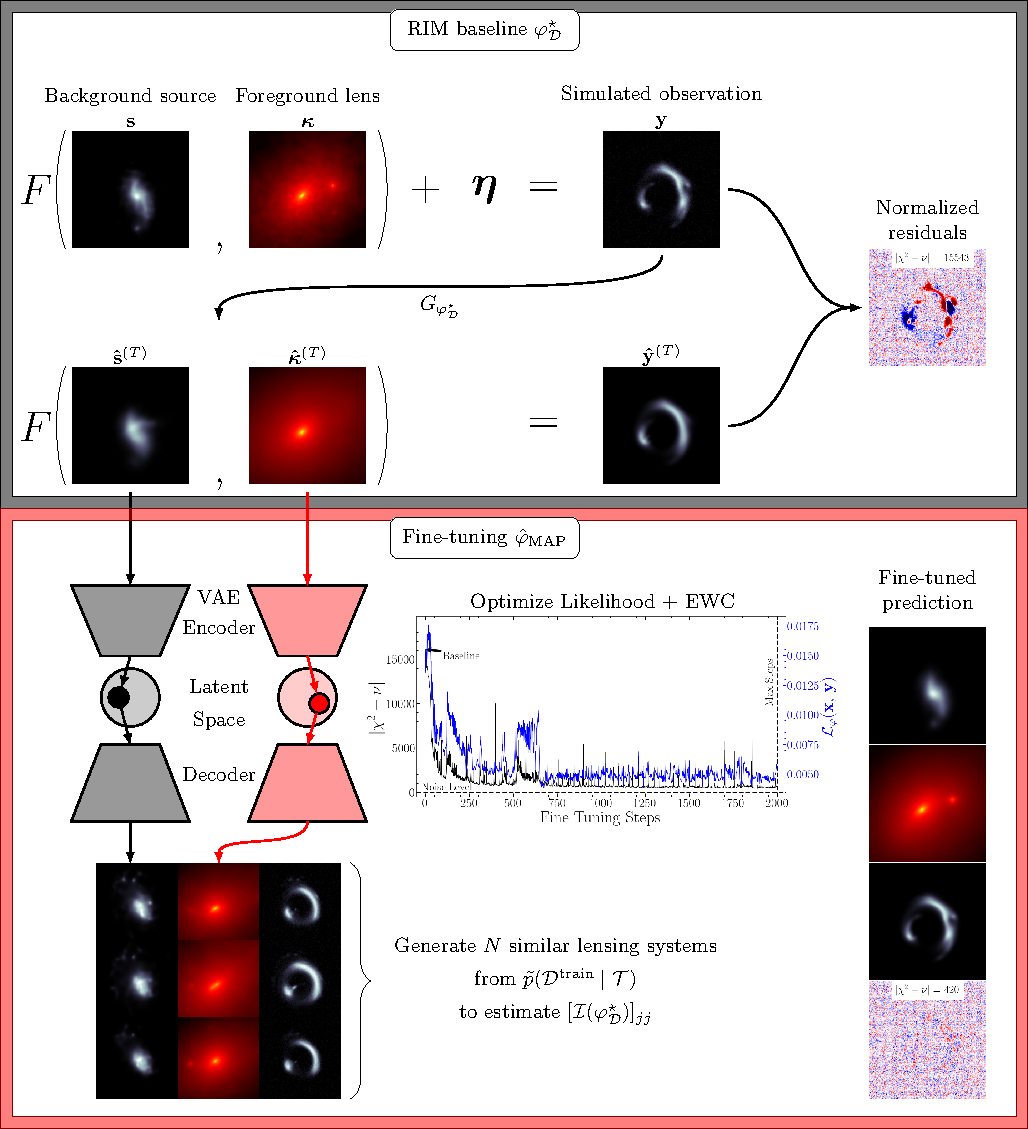
\includegraphics[width=0.9\textwidth]{figures/main_figure}
        %\caption{A summary of the main concepts explored in this paper. First, 
        %a source and convergence map are used to produce a noisy observation. This observation 
        %is the input of the RIM baseline model $G_{\varphi_{\mathcal{D}}^{\star}}$, which 
        %recovers the source and convergence map. The observed data is compared with 
        %the RIM prediction using normalized residual maps. To achieve noise level reconstruction 
        %($\chi^2_\nu \simeq 1$), 
        %the model is fine-tuned by a likelihood optimization regularized by Elastic Weight Consolidation (EWC). 
        %We show the steps 
        %to generate a dataset from the conditional $\tilde{p}(\mathcal{D}^{\mathrm{train}} \mid \mathcal{T})$ 
        %using two VAE and the baseline prediction. 
        %These samples are used to compute the diagonal elements of the 
        %Fisher matrix $[\mathcal{I}(\varphi_{\mathcal{D}}^{\star})]_{jj}$.
%}
        %\label{fig:main figure}
%\end{figure*}



\subsection{Recurrent Inference Machine}\label{sec:rim}

Instead of handcrafting such a distribution, we 
attempt to build an inference machine with
an implicit prior built in the training set $\mathcal{D}$ and 
encoded in a deep neural network architecture \citep{Bengio2009}. 
% We will use the notation $G_{\varphi}$ to make reference to the RIM 
% with parameters $\varphi$. 
The RIM \citep{Putzky2017} is a form of learned 
gradient-based inference algorithm intended to solve inverse problems of the form 
of equation \eqref{eq:MainEquation}. This framework has mainly been applied in the context of linear and under-constrained inverse problems --- i.e. where the function $F$ can be represented in a matrix form and where a prior on the solution space is required to produce a unique solution --- for which the prior on the parameters $\mathbf{x}$, $p(\mathbf{x})$, is 
either intractable or hard to compute \citep{Morningstar2018,Morningstar2019,Lonning2019}. 
The use of the RIM to solve non-linear inverse problems was first investigated in \citep{Modi2021}.
In our case, the inverse problem is non-linear, as it is given by equation (\ref{eq:LensEquation}).


\begin{figure}[tb!]
       \centering 
       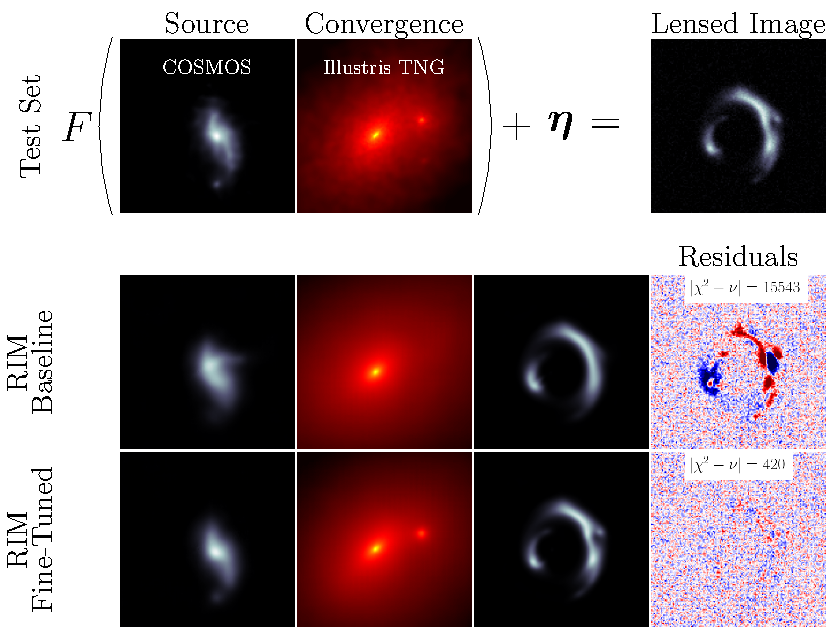
\includegraphics[width=0.7\linewidth]{figures/main_figurev2}
       \caption{Example of a simulated lensed image in the test set that 
exhibits a large deflection in its eastern arc which indicates the presence of a massive object
 --- in this case a dark matter subhalo. The fine-tuning procedure is able to recover 
this subhalo because of its strong signal in the lensed image and reduces the residuals 
to noise level.}
       \label{fig:main figure}
\end{figure}


The governing equation for the RIM is a recurrent 
relation that takes the general form
\begin{equation}\label{eq:RIM}
        \mathbf{\hat{x}}^{(t+1)} = \mathbf{\hat{x}}^{(t)} 
        + g_\varphi \big(\mathbf{\hat{x}}^{(t)},\, \mathbf{y},\, 
\grad_{\mathbf{\hat{x}^{(t)}}} \log p(\mathbf{y} \mid \mathbf{\hat{x}}^{(t)})\big).
\end{equation}
In the text, we will often use the shorthand notation ${\grad_{\mathbf{y} \mid \mathbf{x}} \equiv 
\grad_{\mathbf{x}} \log p(\mathbf{y} \mid \mathbf{x})}$
to refer to the gradient of the likelihood.
By minimizing a weighted mean squared loss backpropagated 
through time, 
\begin{equation}\label{eq:Loss}
		\mathcal{L}_\varphi(\mathbf{x}, \mathbf{y}) = 
		\frac{1}{T}\sum_{t=1}^{T}\sum_{i=1}^{M} \mathbf{w}_i (\mathbf{\hat{x}}^{(t)}_i - \mathbf{x}_i)^2,
\end{equation} 
the neural network $g_\varphi$ learns to optimize the 
parameters $\mathbf{x}$ given a likelihood function. 
The converged parameters of the neural network given the training set $\mathcal{D}$, 
$\varphi^{\star}_{\mathcal{D}}$, are those that minimize the cost --- or empirical risk --- 
which is defined as the 
expectation of the loss over $\mathcal{D}$
\begin{equation}\label{eq:Cost} 
		\varphi^{\star}_{\mathcal{D}} = \underset{\varphi}{\text{argmin}}\,\,
		\mathbb{E}_{(\mathbf{x},\mathbf{y}) \sim \mathcal{D}}\big[
		\mathcal{L}_\varphi(\mathbf{x}, \mathbf{y}) \big].
\end{equation} 
Unlike previous works 
\citep{Andrychowicz2016,Putzky2017,Morningstar2018,Morningstar2019,Lonning2019}, 
the data vector $\mathbf{y}$ --- or observation --- 
is fed to the neural network in order to learn 
the initialization of the parameters ($\mathbf{x}^{(0)} = g_\varphi(0, \mathbf{y}, 0)$) 
as well as their optimization. 
We found empirically that this significantly improves the performance 
of the model for our problem and it avoids situations where 
the model would get stuck in local minima at 
test time due to poor initialization. 
\begin{figure}[t!]
        \centering
		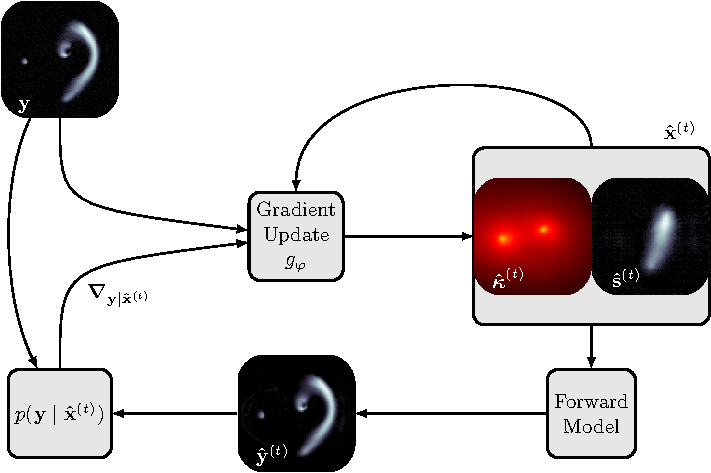
\includegraphics[width=0.6\linewidth]{figures/schematic_rim}
        \caption{Rolled computational graph of the RIM. Dashed arrows represent operations not recorded for BPTT.}
        \label{fig:rolled graph}
\end{figure}


We follow previous works in setting a uniform weight over the time 
steps ($\mathbf{w}^{(t)} = \frac{\mathbf{w}}{T}$). 
The choice of the pixel weights $\mathbf{w}_i$ is informed 
by our empirical observations when training the network. Details 
are reported in appendix \ref{ap:rim training and opt}.

%In figure \ref{fig:unrolled_graph}, we show the unrolled computational graph of the RIM. 
In Figure \ref{fig:rolled graph}, we show the rolled computational graph of the 
RIM. During training of the gradient model $g_\varphi$, operations along the solid arrows are being 
recorded for backpropagation through time. 
The recording is stopped along the dashed arrow since these operations 
are part of the forward modelling process.
By avoiding the computation of these gradients, training time is reduced and 
knowledge about the inner workings  
of a specific likelihood (and forward model) is insulated from the optimization algorithm.
This is analogous to a common RNN use-case like text generation, where the process responsible 
for producing the next element in a time series is a black box to the optimization 
algorithm. 

The gradient of the likelihood is computed using automatic differentiation. Following 
\citep{Modi2021}, we preprocess the gradients using the Adam algorithm \citep{Kingma2013}. 
For clarity, we only illustrated this step in Figure \ref{fig:unet}. 
% \vfill\null

\begin{figure*}[ht!]
        \centering
        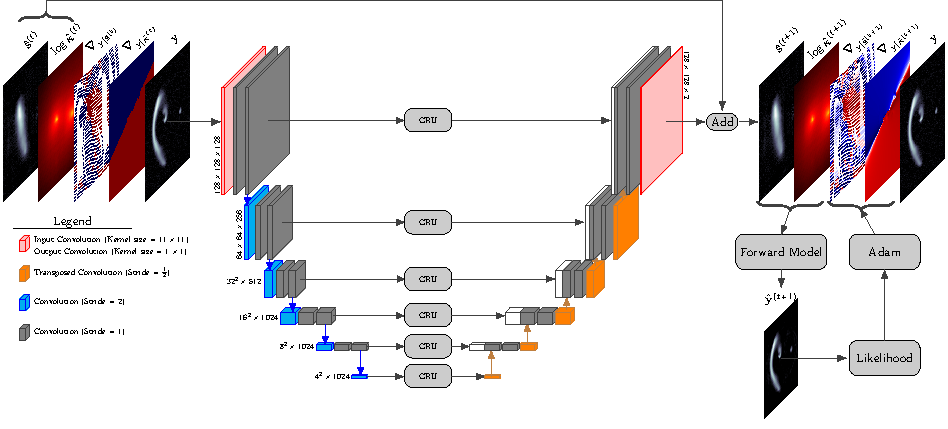
\includegraphics[width=\textwidth]{figures/unet_architecture.pdf}
        \caption{
A single time step of the unrolled computation graph of the RIM.
GRU units are placed in the skip connections to guide the 
reconstruction of the source and convergence. A schematic of the steps to compute 
the likelihood gradients is shown in the bottom right of the figure, including the 
Adam processing step of the likelihood gradient.}
        \label{fig:unet}
\end{figure*}

\subsection{The Gradient Model}\label{sec:gradient model}


The neural network architecture is illustrated in Figure \ref{fig:unet}, which shows 
a single time step of the unrolled computation graph of the RIM.
We use a U-net \citep{Ronneberger2015} architecture 
with Gated Recurrent Units \citep[GRU:][]{Cho2014} placed in each skip connections. 

Each GRU cell has it's own memory tensor that is updated through time at each iteration of 
equation \ref{eq:RIM}. The shape of a memory tensor is set to match the
feature tensor fed into it from the parent layer in the network graph. 
Instead of learning a compressed representation like in the hourglass
architecture (i.e. autoencoder), the U-net architecture naturally separates the spatial 
frequency components of the signal into its vertical levels. The first level generally encodes 
high frequency features while the lower level encodes low frequency features (due to downsampling of the feature maps). 
Adding an independent memory unit 
at each level preserve this property.

Convolutional layers with a stride of 2 are used for downsampling and 
stride of $\frac{1}{2}$ for upsampling of the feature maps 
(identified in blue and orange respectively in figure \ref{fig:unet}). Half-stride convolutions are implemented in practice with the transposed convolution layers from \texttt{Tensorflow} \citep{tensorflow}.
Most layers use a kernel size of $3\times3$, except the first and last layer. 
The first layer has 
larger receptive field ($11\times11$) in order to capture more details in the input tensor. 
The last layer has kernels of size $1\times 1$. 
A $\tanh$ 
activation function is used 
for each convolutional layer, including strided convolutions, except for the output 
layer. The U-net outputs an image tensor with two channels, one dedicated for the update of the source 
and the other to the update of the convergence (see figure \ref{fig:unet}). 
% \vfill\null
%\columnbreak


% Talk about this choice
% Shared memory is important, possibly more than the notion that source and kappa require very different 
% reconstruction procedure (because of different structure etc).

% Choice of model correspond to choosing an inductive bias, or how the function should behave 
% for points in and out of the dataset
% Generalization means the ability to make prediction about the behavior of the function 
% at novel points in the domain of the function.
% In the meta-learning framework, examples are problem instances. Generalization means to transfer 
% knowledge accross problem instances.
% The reuse of the problem structure is known as transfer learning. In the context of meta-learning, 
% this is cast as generalization.

\subsection{The Forward Model}\label{sec:forward model}

An observation is simulated by ray tracing the brightness distribution 
of the background source to the foreground coordinate system. 
In our case, the coordinate systems have discretized representations.
Each pixel of an image is labeled with a subscript index $i$, which 
we distinguish from a parenthesized superscript index $(i)$ that refers to 
the member of a set or list of tensors. For clarity, we omit 
the superscript index in what follows.

Each pixel is associated 
with an intensity value and a coordinate vector.
The foreground pixel coordinates $\boldsymbol{\theta}_i$ and the source 
pixel coordinates $\boldsymbol{\beta}_i$ are related by
the lens equation
\begin{equation}\label{eq:LensEquation}
        \bm{\beta}_i = \bm{\theta}_i - \bm{\alpha}(\bm{\theta}_i),
\end{equation}
where $\boldsymbol{\alpha}$ is a deflection angle.
It is obtained from the projected surface 
density field $\kappa$ --- also referred to as convergence --- by the integral
\begin{equation}\label{eq:alpha}
        \bm{\alpha}(\boldsymbol{\theta}_i) = 
        \frac{1}{\pi} \int_{\mathbb{R}^2}
        \kappa(\boldsymbol{\theta}') 
        %\underbrace{
        \frac{\boldsymbol{\theta}_i
        - \boldsymbol{\theta}'}{\lVert \boldsymbol{\theta}_i - 
        \boldsymbol{\theta}' \rVert^2}
%}_{\displaystyle \boldsymbol{\omega}(\boldsymbol{\theta_i} -\boldsymbol{\theta'})} 
        d^2\boldsymbol{\theta}'.
\end{equation}
The intensity of a pixel in a simulated observation
is obtained by bilinear interpolation of the 
source brightness distribution at the coordinate $\boldsymbol{\beta}_i$.
In this work, the convergence also has a discrete representation. Thus, 
we approximate this integral by a discrete global convolution. Taking 
advantage of the convolution theorem, this operation 
can be computed in near-linear time using 
the Fast Fourier Transform (FFT). 

Assuming the observation 
has $M^2$ pixels, the convolution kernel %$\boldsymbol{\omega}$ 
would have $(2M + 1)^{2}$ pixels. 
Both the convergence tensor and the kernel tensor are zero-padded 
to a size of $(4M+1)^{2}$ pixels in order to approximate a linear 
convolution and significantly reduce aliasing.

A blurring operator --- convolution by a point spread function (PSF) --- is then 
applied to the lensed image to replicate the response of an imaging system. 
This operator is implemented as a GPU-accelerated matrix operation 
since the blurring kernels used in this paper have a significant proportion
of their energy distribution encircled inside a small pixel radius. 
% \vfill\null

\subsection{Fine-Tuning}\label{sec:fine-tuning}

\subsubsection{Objective function}
Once the gradient model is trained, the RIM is a baseline 
estimator of the parameters $\mathbf{x}$ given a noisy observation $\mathbf{y}$, 
a PSF and a noise covariance matrix. 
%We note $(\mathbf{y},\Pi,C) \sim \mathcal{T}$.
We now concern ourselves with a strategy to improve 
this estimator. 
This is important 
for observations with high SNR, for which the estimator
must be extremely accurate to model all the fine features present in the arcs.
The metric for the goodness of fit 
is the reduced chi squared $\chi^2_\nu = \frac{\chi^2}{\nu}$, 
where $\nu$ is the total number of degrees of freedom which corresponds to 
the total amount of pixels in $\mathbf{y}$ in this work.
Generally, our goal will be to reach $\chi^2_\nu = 1$, or equivalently $|\chi^2 - \nu| = 0$, 
which indicates that the RIM hypothesis has reconstructed all the signal 
to be recovered from the observation. 
We note that such a problem is exceedingly  
difficult at high SNR. In this regime, 
our hypothesis has 
to be both precise and accurate in order to satisfy the chi squared test. 
This is unlike noisy observations, where strong assumptions about the model 
parameters are required and often sufficient to reconstruct the 
remaining information left in the observed vector $\mathbf{y}$.

We observe that we can optimize the network parameters w.r.t to the 
chi squared directly
\begin{equation}\label{eq:MAP} 
        \hat{\varphi}_{\mathrm{MAP}} = \underset{\varphi}{\mathrm{argmax}}\,\, 
        \frac{1}{T}\sum_{t=1}^{T} \log p(\mathbf{y} \mid \mathbf{\hat{x}}^{(t)}) + \log p(\varphi).
\end{equation} 
Unlike the loss in equation \eqref{eq:Loss}, this objective function makes no use of labels 
($\mathbf{x}$). 
This allows us to use equation \eqref{eq:MAP} at test time in order to fine-tune the RIM's weights to a specific test example. 

\subsubsection{Transfer Learning}
We now address the issue of transferring knowledge from the training task, problem \eqref{eq:Cost}, 
to a test task specific to an observation, problem \eqref{eq:MAP}.
The reader might refer to reviews on transfer learning \citep{Pan2010,Zhuang2019} 
for a broad overview of the field. The strategy we outline fall into 
the category of inductive transfer learning.

Since the data likelihood $p(\mathbf{y} \mid \mathbf{x})$ 
does not contain \textit{a priori} information 
about the solution $\hat{\varphi}_{\mathrm{MAP}}$,
inductive biases must be introduced to make 
the problem \eqref{eq:MAP} well-posed. Thus, we
\begin{enumerate}[label=(\subscript{\mathcal{H}}{{\arabic*}})]
        %\setcounter{enumi}{3}
        \item \label{prior:initialization} initialize the network parameters with $\varphi_{\mathcal{D}}^{\star}$; 
        \item \label{prior:early stopping} apply early stopping when a maximum number of steps is reached or 
                $\chi^2_\nu \leq 1$;
        \item \label{prior:learning rate} use a small learning rate.
\end{enumerate}
\ref{prior:early stopping} and \ref{prior:learning rate} encode the assumption 
that the optimal estimator is to be found \textit{near} the initialization.

As it turns out, \ref{prior:initialization} is not strong 
enough to preserve the knowledge learned from the training task. 
This has long been observed in the literature and was coined as the 
catastrophic interference phenomenon in 
connectionist networks \citep{McCloskey1989,Ratcliff1990}.
In summary, a sequential learning problem exhibits catastrophic 
forgetting of old knowledge when confronted with new examples (possibly 
from a different distribution or process), in a manner 
\begin{enumerate}[label=(\subscript{\mathrm{CF}}{{\arabic*}})]
        \item \label{cf:steps} proportional to the amount of learning;
        \item \label{cf:weights} strongly dependant to the disruption of the parameters
                involved in representing the old knowledge.
\end{enumerate}
While \ref{prior:early stopping} and \ref{prior:learning rate} can 
potentially alleviate \ref{cf:steps}, \ref{cf:weights} is not 
trivially addressed by the inductive biases introduced so far.

\begin{figure}[t!]
        \centering
        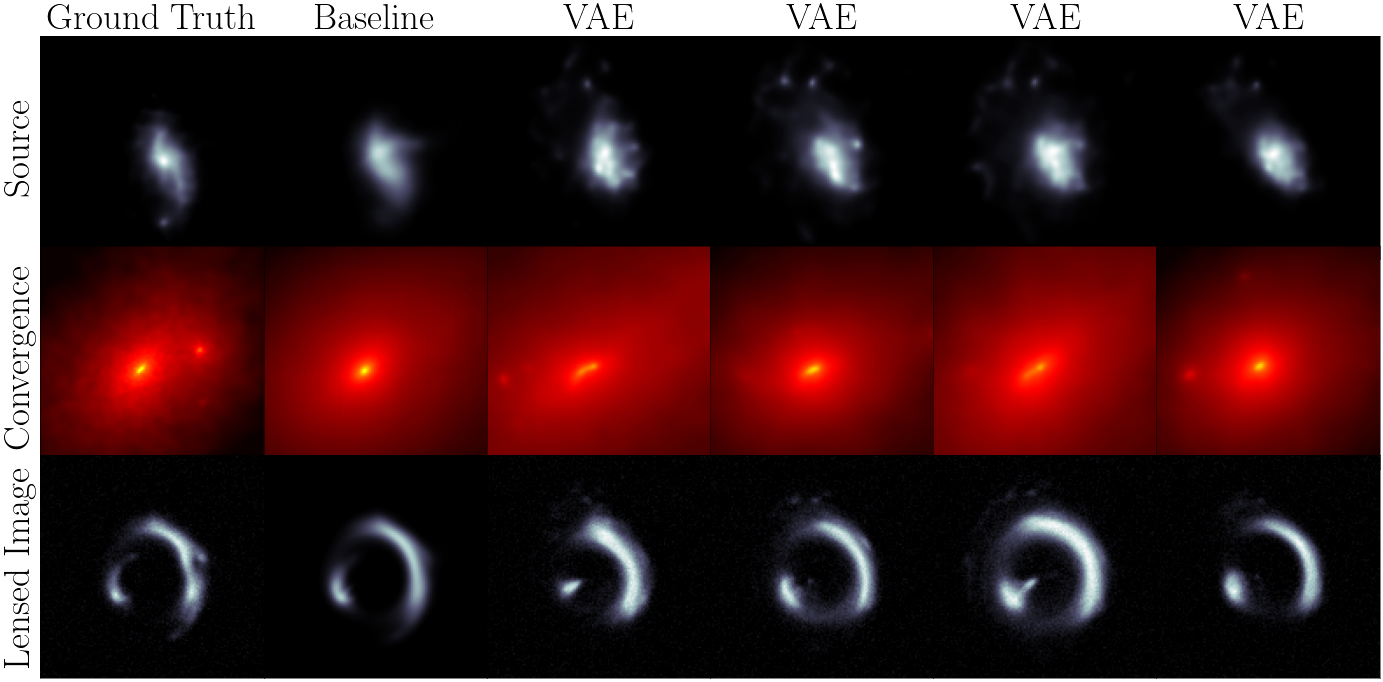
\includegraphics[width=0.8\linewidth]{figures/vae_samples_similar_to_highlight}
        \caption{Examples similar to the test task, also shown in Figure \ref{fig:main result}. The first column shows the ground truth used to simulate the lensed image. The second column shows the baseline prediction that is then encoded in the latent space of the VAE in order to sample the next 4 columns.
}
        \label{fig:vae fine-tuning}
\end{figure}

We follow the work of \citet{Kirkpatrick2016} to define a prior distribution
over $\varphi$ that address this issue
\begin{equation}\label{eq:Prior} 
        \log p(\varphi) \propto -\frac{\lambda}{2}\sum_{j} \mathrm{diag}(\mathcal{I}(\varphi_{\mathcal{D}}^{\star}))_{j} 
        (\varphi_j - [\varphi^{\star}_{\mathcal{D}}]_{j})^{2}\, .
\end{equation} 
$\mathrm{diag}(\mathcal{I}(\varphi_{\mathcal{D}}^{\star}))$ is the diagonal of the 
Fisher information matrix 
encoding the amount of information that  
some set of gravitational lensing systems from 
the training set, and similar to the observed 
test task, carries about the baseline RIM weights $\varphi_{\mathcal{D}}^{\star}$ 
--- the parameters that minimize the empirical risk (equation \ref{eq:Cost}).
We can also understand this prior using the
Cramér-Rao lower bound 
\citep{Rao1945,Cramer1946}.
%\begin{equation}\label{eq:iCramerRao}
        %\mathrm{Var(\varphi)} \geq \underbrace{(1 + \mathrm{Bias}_{\mathcal{D}}(\varphi))^{2}}_{\lambda_b}\mathcal{I}(\varphi)^{-1}.
%\end{equation} 
The prior can thus be framed as a multivariate 
Gaussian distribution characterised by a diagonal covariance matrix with $\mathrm{diag}(\mathcal{I})$ as its inverse 
and by $\varphi^{\star}_{\mathcal{D}}$ as its first moment.
Within this view, the  
Lagrange multiplier is 
tuning our estimated uncertainty about the neural network weights 
for the particular task at hand.  
We've included a derivation 
of this term in the appendix \ref{ap:ewc}.


%We define the distribution of examples from $\mathcal{D}$ similar to the test task $\mathcal{T}$ with 
%the surrogate conditional $\tilde{p}(\mathcal{D} \mid \mathcal{T})$. 
Examples are drawn from the set of training examples similar to the test task 
by sampling the latent space of both the source 
VAE and the convergence VAE near the baseline prediction of the RIM. Figure \ref{fig:vae fine-tuning} illustrates what we mean by \textit{similar}. 


%By definition, the Fisher matrix is the 
%expected value of the observed information that 
%the examples carry about $\varphi$. 

%We can, however, make use of theoretical and 
%experimental evidence that overparametrized 
%neural networks exhibits a spectral bias \citep{Rahman2018} 
%toward learning low frequencies first during training. We observe 
%that the baseline model generally 
%provides a coherent prediction ($\gamma(k) = 1$) in the low frequency 
%regime, which is consistent with a spectral bias hypothesis. 
%This suggest a possible approach to ground our method. 
%The MLE-optimal estimator should at least 
%preserve the low frequency features predicted by the baseline. 
%Otherwise, we might suspect that the optimisation procedure 
%has found a degenerate solution that is not consistent with the 
%prior learned by the baseline.

%This also points to interesting strategies that could alleviate 
%overfitting. For instance, freezing the deeper layers of the U-net during 
%fine-tuning might preserve the low frequency features learned during pretraining. 
%This is also suggested as a strong regularization method in \citet{Li2018}. 
%We explore such ideas in the appendice


\section{Data}\label{sec:data}

\subsection{COSMOS}\label{sec:source}
The background source brightness distributions are taken from the Hubble Space Telescope (HST) 
Advanced Camera for Surveys Wide Field Channel COSMOS field \citep{Koekemoer2007,Scoville2007},
a $1.64\,\mathrm{deg}^{2}$ contiguous survey acquired in the F814W filter. 
A dataset of mag limited ($\mathrm{F814W} < 23.5$) deblended galaxy postage stamps \citep{Leauthaud2007} was compiled as 
part of the GREAT3 challenge \citep{Mandelbaum2014}. The data is 
publicly available \citep{Mandelbaum2012}, and the preprocessing is done through the open source software 
\texttt{GALSIM} \citep{Rowe2015}. \par

We applied the 
\texttt{marginal} selection criteria (see the \texttt{COSMOSCatalog} class) and imposed a flux per image
greater than $50\,\,\mathrm{photons}\,\,\mathrm{cm}^{-2}\,\mathrm{s}^{-1}$. 
This final set has a total of 13\,321 individual images.
Each image is convolved with its original PSF and drawn into a postage stamps of $158^2$ pixels. 
Each image is then 
background subtracted, randomly shifted, rotated by an angle multiple of $90^\circ$, cropped 
cropped down to $128^{2}$ pixels and normalized to pixel intensities in the range $[0,1]$.

We split each unique galaxies into a training set (90\%) and a test set (10\%). 
The training set is used to train a VAE and produce simulated observations 
to train the RIM.

\begin{figure}[t!]
        \centering
        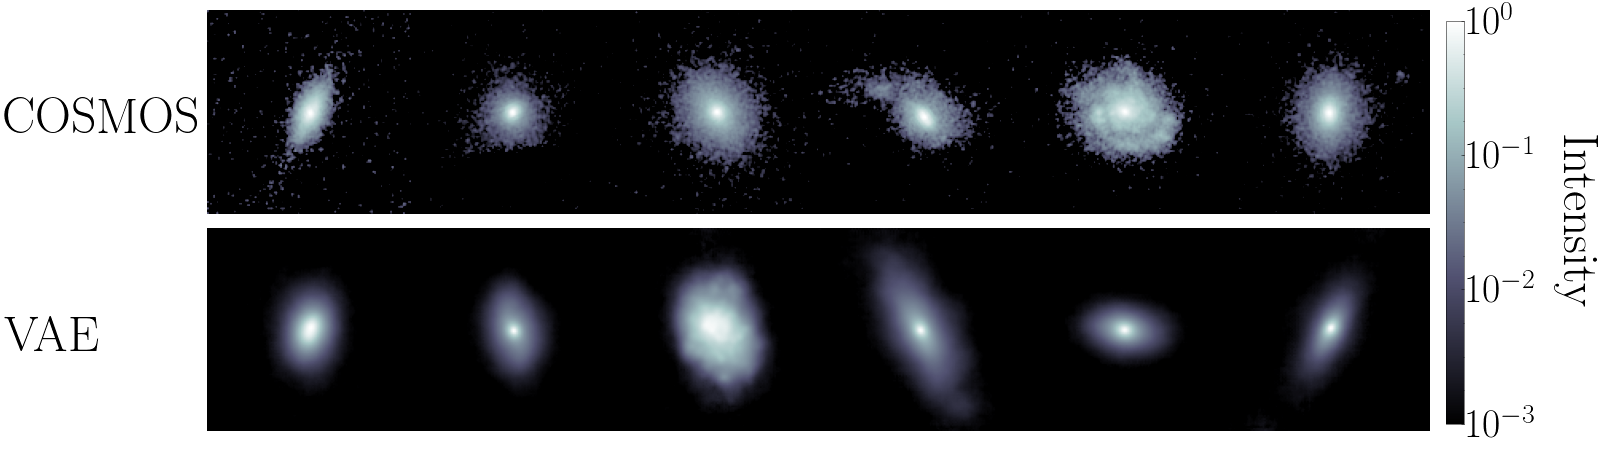
\includegraphics[width=0.7\linewidth]{figures/gal_vae_sample}
        \caption{Examples of COSMOS galaxy images 
                (top row) and VAE generated samples (bottom row) used as labels in $\mathcal{D}$.}
        \label{fig:source}
\end{figure}


\subsection{IllustrisTNG}\label{sec:kappa}
\subsubsection{Smooth Particle Lensing}\label{sec:SPL}
To compute a convergence map from an N-body simulation, 
we follow \citet{Auger2007} in treating 
each particle as flow tracers instead of describing their density as Dirac delta functions. 
Smoothing each particle density on a non-singular kernel reduces the particle noise affecting all 
important lensing quantities --- most importantly the convergence. At the same time, the choice of the kernel size 
is important to preserve substructures in the 
lens that we might potentially be interested in. Following \citet{Rau2013}, we use Gaussian 
smoothing with an adaptive kernel size determined by the distance of the 64\textsuperscript{th} nearest neighbours of 
a given particle $D_{64,i}$. 
\begin{equation}\label{eq:Ksmooth}
\begin{aligned}
    \kappa(\mathbf{x}) &= \frac{1}{\Sigma_{\mathrm{crit}}} \sum_{i=1}^{N_{\mathrm{part}}}
        \frac{m_i}{2 \pi \hat{\ell}^2_i} 
        \exp \left(-\frac{1}{2} \frac{(\mathbf{x} - \mathbf{x}_i)^2}{\hat{\ell}_i^2}  \right) \\
    \hat{\ell}_i &= \sqrt{\frac{103}{1024}}D_{64,i}.
\end{aligned}
\end{equation}
The nearest neighbours are found by fitting a k-d tree ---  implemented in 
\texttt{scikit-learn} \citep{scikit-learn} --- 
to the $N_{\mathrm{part}}$  particles 
in a cylinder centered on the centre of mass of the halo of interest.
The critical surface density is defined as
\begin{equation}\label{eq:Scrit}
\Sigma_{\mathrm{crit}} = \frac{4 \pi G}{c^ 2} \frac{D_\ell D_{\ell s}}{D_s},
\end{equation}
where $D_\ell$, $D_s$ and $D_{\ell s}$ are angular diameter distance to the lens, source and between the lens and the source respectively, 
$G$ is the gravitational constant and $c$ the speed of light.

\subsubsection{Preprocessing}
The projected surface density maps (convergence) of lensing galaxies 
were made using the redshift $z=0$ snapshot  
of the IllustrisTNG-100 simulation \citep{Nelson2018} 
in order to produce physically realistic realizations of dark matter and baryonic matter halos.
We selected 1604 halos with the criteria that they have a total
dark matter mass of at least $9\times10^{11} M_{\odot}$. We then collected all 
dark matter, gas, stars and black holes particles from the data associated to the galaxy 
cluster within which the halo resides in to create a smoothed projected surface density maps 
around the centroid of the halo as prescribed in section \ref{sec:SPL}.

\begin{figure}[t!]
        \centering
        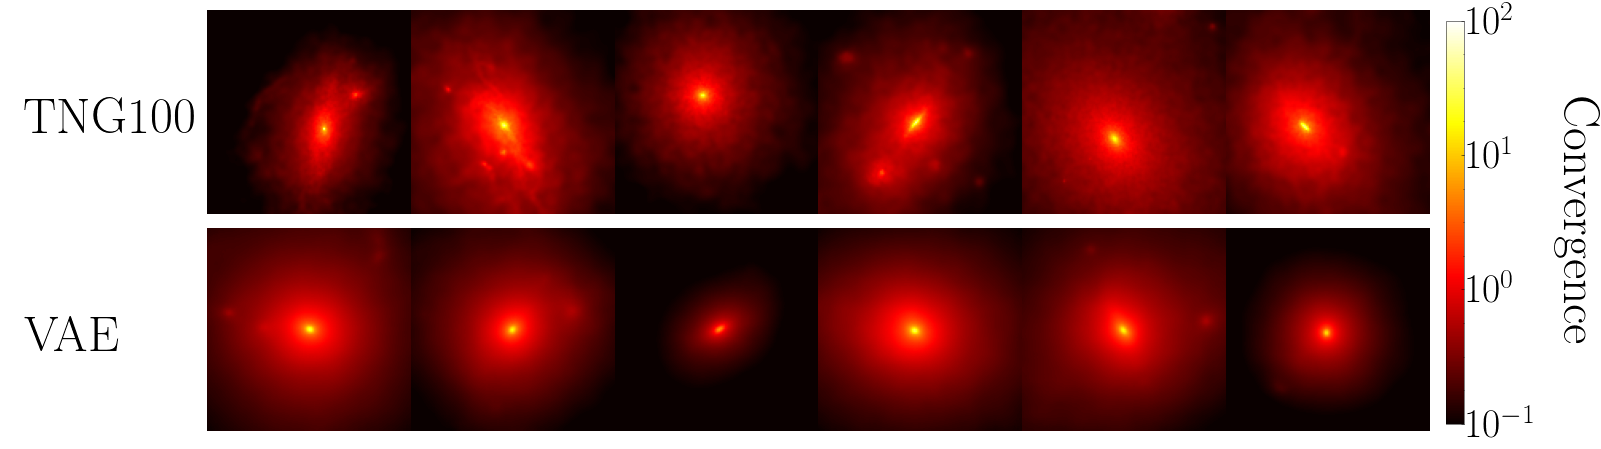
\includegraphics[width=0.7\linewidth]{figures/kap_vae_sample}
        \caption{Examples of smoothed Illustris TNG100 convergence map (top row) 
        and VAE generated samples (bottom row) used as labels in $\mathcal{D}$.}
        \label{fig:kappa}
\end{figure}

We adopt the $\Lambda$CDM cosmology from 
\citet{PlanckCollaboration2018} with $h=0.68$ to compute 
angular diameter distances. We also fix the 
source redshift to $z_s=1.5$ and the deflector redshift to $z_\ell=0.5$. 
We note that changing the redshifts or the cosmology 
only amount in a rescaling of the $\kappa$ map by a global scalar, not 
the morphology of the profiles. Thus, this choice does not change the generality of our method.
The smoothed distributions from equation \eqref{eq:Ksmooth} are 
rendered into a regular grid of $188^2$ pixels with a comoving field of view of $105\,\,\mathrm{kpc}/h$. 
To avoid 
edge effects in the pixelated maps, 
we include particles outside of the field of view in the sum of equation \eqref{eq:Ksmooth}.
\par
Before applying augmentation or considering different projections, our dataset of halos is split into a 
training set (90\%) and a test set (10\%) in order to make sure that the test set consists only 
of convergence maps unseen by the RIM during training.
We take 3 different projections ($xy$, $xz$ and $yz$) of each 3D particle 
distributions, which amounts to a dataset with a total of $4\,812$ individual convergence maps. 
Random rotations by an angle multiple of $90^{\circ}$ and random shifts to the pixel coordinates 
are applied to each image. The $\kappa$ maps are then rescaled by a random factor to change their 
estimated Einstein radius to the range 
$[0.5,\,2.5]$ seconds of arc.
The Einstein radius is defined as
\begin{equation}\label{eq:ThetaE}
        \theta_E = \sqrt{\frac{4GM(\theta_E)}{c^ 2} \frac{D_{\ell s}}{D_\ell D_s}}
\end{equation} 
where $M(\theta_E)$ is the mass enclosed inside the Einstein radius. In practice, we estimate this quantity 
by summing over the mass of pixels with a value greater than the critical density ($\kappa > 1$). 
For data augmentation purposes, this procedure gives a good enough estimate of the 
size of the lensed image that will be produced by some $\kappa$ map. 
We test multiple scaling factors for each $\kappa$ map, then uniformly sample between those that produce an estimated 
Einstein radius within the 
desired range. This step is used to remove any bias in the Einstein radius that might come from the mass function 
of the simulation.

The final maps are cropped down to $128^2$ pixels.
Placed at a redshift $z_\ell=0.5$, a $\kappa$ map will thus span an angular field of view of $7.69''$ with 
a resolution similar to HST. 
%This field of view is wide enough to cover a typical gravitational 
%lens observed in the sky, which partly justify our choice for the comoving field of view earlier. 
With these augmentation procedures, a total of $50\,000$ maps are created from the training split and 
$5\,000$ from the test split.
The training set is used to train a VAE and produce simulated observations 
to train the RIM. 

\subsection{Simulated Observations}\label{sec:simulated observation}
Having defined a source map and a convergence map, we apply the ray tracing simulation 
prescribed in section \ref{sec:forward model} to produce an observation 
with observational effects that crudely correspond to HST images. 

For each observation, a Gaussian point spread function is 
created with a full width at half maximum (FWHM) 
randomly generated from a truncated normal distribution.
The support of the distribution is truncated below by the 
angular size of a single pixel and above by the angular size of 4 pixels. 
White noise with a standard deviation randomly generated from a truncated normal distribution 
is then added to the convolved observation to simulate SNR conditions between 
$10\,\mathrm{dB}$ and $30\,\mathrm{dB}$. For simplicity, we define $\mathrm{SNR} = \frac{1}{\sigma}$. 
This definition is equivalent to the peak signal-to-noise ratio. 

%We set the observed image field of view to match with the convergence field view ($7.69''$). 
%We choose the background field of view to be $3''$.
As a validation criteria for each simulated image, we impose 
a minimum magnification of 3. Thus, 
we make sure that most pixel coordinates in the image plane will be mapped inside the 
source coordinate system through the lens equation \eqref{eq:LensEquation}. 

\begin{table}[htb!]
\centering
\begin{threeparttable}
\caption{Physical model parameters.}
\label{tab:phys}
\begin{tabular}{ccc}
        Parameter &  Distribution/Value \\
        \hline \hline
        Lens redshift $z_\ell$ & $0.5$ \\
        Source redshift $z_s$ & $1.5$ \\
        Field of view ('') & $7.69$ \\
        Source field of view ('') & $3$ \\
        PSF FWHM ('') & $\mathcal{TN}(0.06,\, 0.3;\, 0.08,\, 0.05)$\tnote{*}\\
        Noise amplitude $\sigma$ & $\mathcal{TN}(0.001,\, 0.1;\, 0.01,\,0.03)$\tnote{*}\\
        \hline
\end{tabular}
\begin{tablenotes}\footnotesize
\item[*]We defined the parameters of the truncated normal in the order $\mathcal{TN}(a,\, b;\, \mu,\, \sigma)$, where $[a,\, b]$ defines the support of the distribution.
\end{tablenotes}
\end{threeparttable}
\end{table}

$400\,000$ observations are simulated from random pairs of COSMOS sources 
and IllustrisTNG convergence training splits in order to train the RIM. 
An additional $200\,000$ observations are created from pairs 
of COSMOS source and pixelated SIE convergence map. 
The parameters for these $\kappa$ maps are listed in table \ref{tab:sie}. 
We found this addition to be beneficial to learning since it adds an 
inductive bias in the learning favoring isothermal profiles.
We expect some lensing configurations like 
large Einstein rings or double images to poorly constrain the inner structure of the 
mass distribution. 
Building an inference pipeline with strong constraints on the 
slope of the profile, other than the lensed image, goes beyond the scope of this work. 
As such, imposing an implicit prior for the slope through 
the dataset is sufficient for our goal. 
It is also motivated by the \textit{bulge-halo conspiracy} --- 
the observation that most lensing configurations observed in the sky can be explained 
to first order approximation by 
an average slope consistent with an isothermal profile \citep{Auger2010,Dutton2014}.

\begin{table}[htb!]
\centering
\caption{SIE parameters.}
\label{tab:sie}
\begin{tabular}{ccc}
        Parameter &  Distribution \\
        \hline \hline
         Radial shift ('') & $\mathcal{U}(0, 0.1)$ \\
        Azimutal shift & $\mathcal{U}(0, 2\pi)$ \\
        Orientation & $\mathcal{U}(0, \pi)$ \\
        $\theta_E$ ('') & $\mathcal{U}(0.5, 2.5)$ \\
        Ellipticity & $\mathcal{U}(0, 0.6)$ \\
        \hline
\end{tabular}
\end{table}


$1\,600\,000$ simulated observations are generated from the VAE 
background sources and convergence maps as part of the training set. 
In principle, we could continuously generate examples from the VAE. 
However, having a fixed amount let us apply some validation check to each 
examples in order to avoid configurations like a
single image of the background 
source or an Einstein ring cropped by the field of view.




\section{Training}\label{sec:training}

\subsection{VAE}\label{sec:vae training}

As mentionned in \citet{Kingma2019}, direct optimisation 
of the ELBO can prove difficult because the reconstruction term $\log p_\theta (\mathbf{x} \mid \mathbf{z})$ 
is relatively weak compared to the Kullback Leibler (KL) divergence term. To alleviate this issue, 
we follow the work of \citet{Bowman2015} and \citet{Sonderby2016} in setting a warm-up 
schedule for the KL term in thstarting from $\beta=0.1$ up to $\beta_{\mathrm{max}}$. 

Usually, 
$\beta_{\mathrm{max}} = 1$ is considered optimal since it matches the original ELBO  
objective derived by \citet{Kingma2013}. 
But, we are more interested in the 
sharpness of our samples and accurate inference around small regions of the latent 
space for fine-tuning. Thus, setting $\beta_{\mathrm{max}} < 1$ allows us to increase 
the size of the information bottleneck (or latent space) of the VAE 
and improve the reconstruction cost of the model. 
This is a variant of the $\beta$-VAE \citep{Higgins2017}, where $\beta > 1$ was found 
to improve disentangling of the latent space \citep{Burgess2018}. 

The value for $\beta_\mathrm{max}$ and the steepness of the schedule 
are grid searched alongside the architecture for the VAE. Our criteria 
for an optimal model is a VAE that achieve the lowest reconstruction error 
in order to produce sharp images. At the same time, the 
KL divergence value should be smaller than an empirically defined threshold to respect 
the latent space prior. 
This value is found in practice by 
manually looking at the quality of generated samples for different VAE 
hyperparameters. A similar method is explored and formalized in the 
InfoVAE framework \citep{Zhao2017}.


A notable element of the VAE architecture is the use of a fully connected  
layer to reshape the features of the convolutional layer into the chosen 
latent space dimension. Following the work of \citet{Lanusse2021}, we introduce 
an $\ell_{2}$ penalty between the input and output of the bottleneck 
dense layers to encourage an identity mapping. This regularisation 
term is slowly removed during training.
%\vfill\null
%\columnbreak

\subsection{RIM}\label{sec:rimtraining}

The architecture of the gradient model was grid searched on 
smaller dataset ($\lesssim 10\,000$ examples) 
in order to quickly identify a small grid 
of valid hyperparameters. Then, the best hyperparameters were 
identified using a two-stage training process on the training dataset. 
In the first stage, we trained 24 different architectures from this small 
hyperparameter set for approximately 4 days (wall time using a single Nvidia A100 gpu). 
Different architectures would have a training time much longer than others, and this 
was factored in the architecture selection process. For example, adding more time 
steps ($T$) to the recurrent relation \eqref{eq:RIM} 
would yield better generalisation on the test set, but this 
would come at great costs to training time until convergence. 
Following this first stage, 4 architectures were deemed efficient enough 
to be trained for an additional 6 days. 
We only report the results for the best architectures out of these 4.
%We report the hyperparameters for 
%the best architecture after this second stage of training in table \ref{tab:baseline hparams}.

\begin{table}[ht!]
\centering
\begin{threeparttable}
        \caption{Hyperparameters for fine-tuning the RIM.}
        \label{tab:fine-tuning hparams}
        \begin{tabular}{cc}
                Parameter & Value \\\hline\hline
                Optimizer & RMSProp \\
                Learning rate & $10^{-6}$\\
                Maximum number of steps & $2\,000$\\
                $\lambda$ & $2\times 10^{5}$\\
                $\ell_2$ & 0 \\
                Number of samples from VAE & 200 \\
                Latent space distribution & $\mathcal{N}(\mathbf{z}^{(T)}, \sigma=0.3)$\tnote{*}\\
                \hline
        \end{tabular}
\begin{tablenotes}\footnotesize
\item[*]$\mathbf{z}^{(T)}$ is the latent code of the RIM baseline source or convergence.
\end{tablenotes}
\end{threeparttable}
\end{table}

Each reconstruction is performed by fine-tuning the baseline model 
on a test task composed of an observation vector, a PSF and a noise covariance.
In practice, fine-tuning the test of $3\,000$ examples can be accomplished in parallel so as to be done in at most a few days by spreading the computation on $\sim 10$ Nvidia A100 GPUs (or 10 hours on $\sim 100$ GPUs). Each reconstruction uses at most 2000 steps, which turns out to be approximately $20$ minutes (wall-time) per reconstruction. Early stopping is applied when the $\chi^2$ reaches noise level. The hyperparameters for this procedure are reported in Table \ref{tab:fine-tuning hparams}.
% Despite this seemingly extreme computational cost, we note that our approach is unique 
% in that it can reconstruct such a large amount of diverse non-parametric systems with the level 
% of precision reported in section \ref{sec:results}. To the knowledge of the 
% authors, no other method can accomplish this task, let alone in less than a week. 
%\vfill\null



\section{Results}\label{sec:results}


In this section, we present the performance of our approach 
on the held out test set. A sample of 3000 reconstruction 
problems is generated from the held-out HST and IllustrisTNG data 
with noise conditions and PSFs similar to the training set.

\subsection{Goodness of Fit}
Figure \ref{fig:main result} is a cherry picked sample of the reconstruction from the test set. 
The samples are selected to showcase the wide range of lensing configuration that 
our approach can successfully solve at high SNR. We made a point to select mostly 
examples that have a lot of structure in their convergence map to distinguish 
our approach from existing analytical methods. We did not make an 
emphasis in selecting complicated sources since we judge that 
free-form reconstruction of the source is essentially a solved problem. 
Indeed, many methods can reconstruct free-form sources 
once the convergence map is known or well constrained 
\citep{Warren2003,Suyu2006,Vegetti2009,Birrer2018,Morningstar2019,Galan2021,Karchev2022,Mishra-Sharma2022}.

To offset our selection bias, we selected samples in different percentile from the
test set rank ordered by the $\chi^2$ metric. 
We also show a randomly selected sample from the test set in Figure \ref{fig:random sample}.

\begin{figure}[th!]
        \centering
        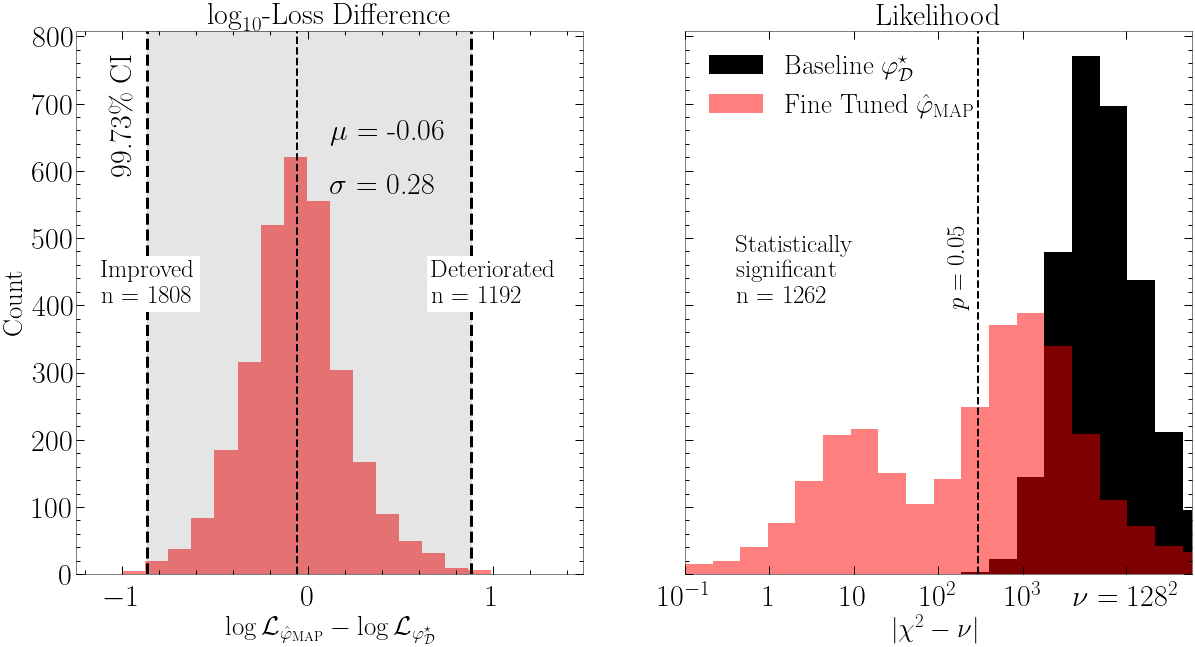
\includegraphics[width=0.8\textwidth]{figures/loss_and_likelihood}
        \caption{Distribution of the goodness of fit for the baseline and fine-tuned network (right panel), as well as log-loss difference between the two network for a given example in the test set (left panel).
        % The 
        % $\chi^2$ is significantly improved by the optimisation. The log-loss difference is 
        % found to have a scatter $\sigma = 0.28$ smaller than the intrinsic scatter of the baseline 
        % log-loss $\sigma(\log \mathcal{L}(\varphi^\star_{\mathcal{D}})) = 0.36$ (see Table \ref{tab:loss}) because of the regularisation by EWC.
}
        \label{fig:loss and chi squared}
\end{figure}


Figure \ref{fig:loss and chi squared} shows a comparison between 
the goodness of fit of the baseline model and the fine-tuned prediction. 
Since we empirically observe that the distribution of the loss on the test set (and the training set) follows a log-normal distribution, we find much more informative to look at the $\log$-loss 
distribution to extract information about the fine-tuning procedure. 
The left panel of Figure \ref{fig:loss and chi squared} 
shows the distribution of the log-loss difference between the fine-tuned prediction and the baseline model. This distribution shows that the fine-tuning procedure loss is constrained within $\sim 1$ order of magnitude of the original loss with a $99.73\,\%$ probability. We find that the log-loss difference has a scatter of $\sigma = 0.28$, which is smaller than the scatter of the baseline log-loss over the entire test set $\sigma(\log \mathcal{L}(\varphi^\star_{\mathcal{D}})) = 0.36$ reported in Table \ref{tab:loss}.
We note that this metric is not optimized during fine-tuning, 
and is only computed as an oracle metric --- still, the fine-tuning procedure does not significantly deteriorate or improve the loss of the baseline prediction in average. We report the first 2 moments of the loss log-normal distribution for the baseline and the fine-tuned reconstructions in Table \ref{tab:loss} in order to compare explicitly the loss distributions. As can be seen in this table, there is no significant difference between the two distribution. This statement can be proven for the measured mean values --- $\mu(\log \mathcal{L}(\hat{\varphi}_{\mathrm{MAP}})) = \mu(\log \mathcal{L}(\varphi^{\star}_{\mathcal{D}})) $ --- using the two-sided normal p-value test \citep{Casella2001}, which we find satisfy the null hypothesis with $p=0.87288$ ($Z = -0.16$). All those observations support our claim that EWC regularisation preserves the prior learned during pretraining, or at least that it preserves the surrogate measures of the prior we reported. 


\begin{table}[th!]
    \centering
    \caption{$\log_{10}$-normal moments of the loss on the test set}
    \label{tab:loss}
    \begin{tabular}{ccc}
        \hline
          Model  & $\mu(\log \mathcal{L})$ & $\sigma(\log \mathcal{L})$ \\
        \hline \hline
        Baseline ($\varphi_{\mathcal{D}}^\star)$ &  -1.96 & 0.36 \\
        Fine-tuned ($\hat{\varphi}_{\mathrm{MAP}}$) & -2.02 & 0.37 \\\hline
    \end{tabular}

\end{table}

\begin{figure}[th!]
        \centering
        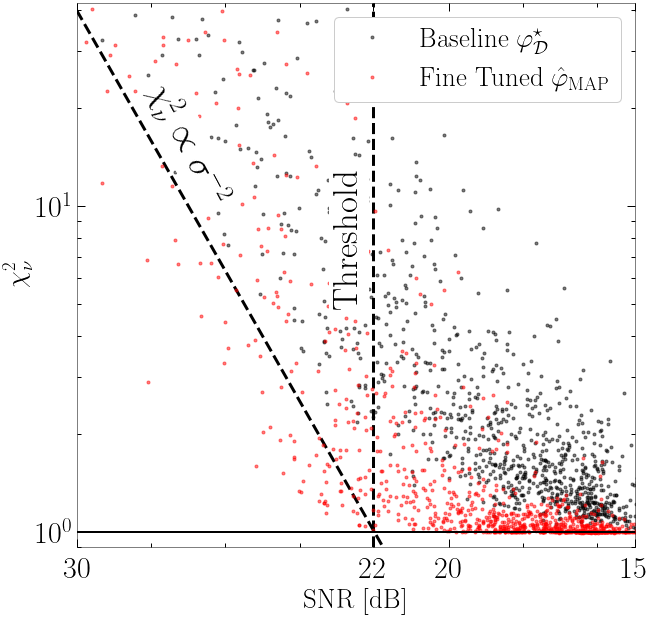
\includegraphics[width=0.6\textwidth]{figures/chisq_vs_noise_ewc}
        \caption{Goodness of fit as a function of SNR shows a threshold 
        behavior where our method reaches its limit.}
        \label{fig:chi squared vs noise}
\end{figure}

The right panel of Figure \ref{fig:loss and chi squared} shows that 
the $\chi^2$ of the reconstruction is improved substantially compared to the 
baseline model. The $\chi^2$ is directly optimized by the fine-tuning procedure 
(equation \eqref{eq:MAP}). Thus, this improvement is to be expected. 
Out of the 
3000 reconstructions, 1262 reach $|\chi^2 - \nu| \leq 296$, which is the criteria 
that satisfy the null hypothesis for the number of degrees of freedom 
$\nu=128^{2}$. For those reconstructions that do not satisfy this criteria, 
we still observe a significant improvement in the distribution of goodness of fit 
compared to the baseline (black histogram in Figure \ref{fig:loss and chi squared}).




\begin{figure}[H]
        \centering
        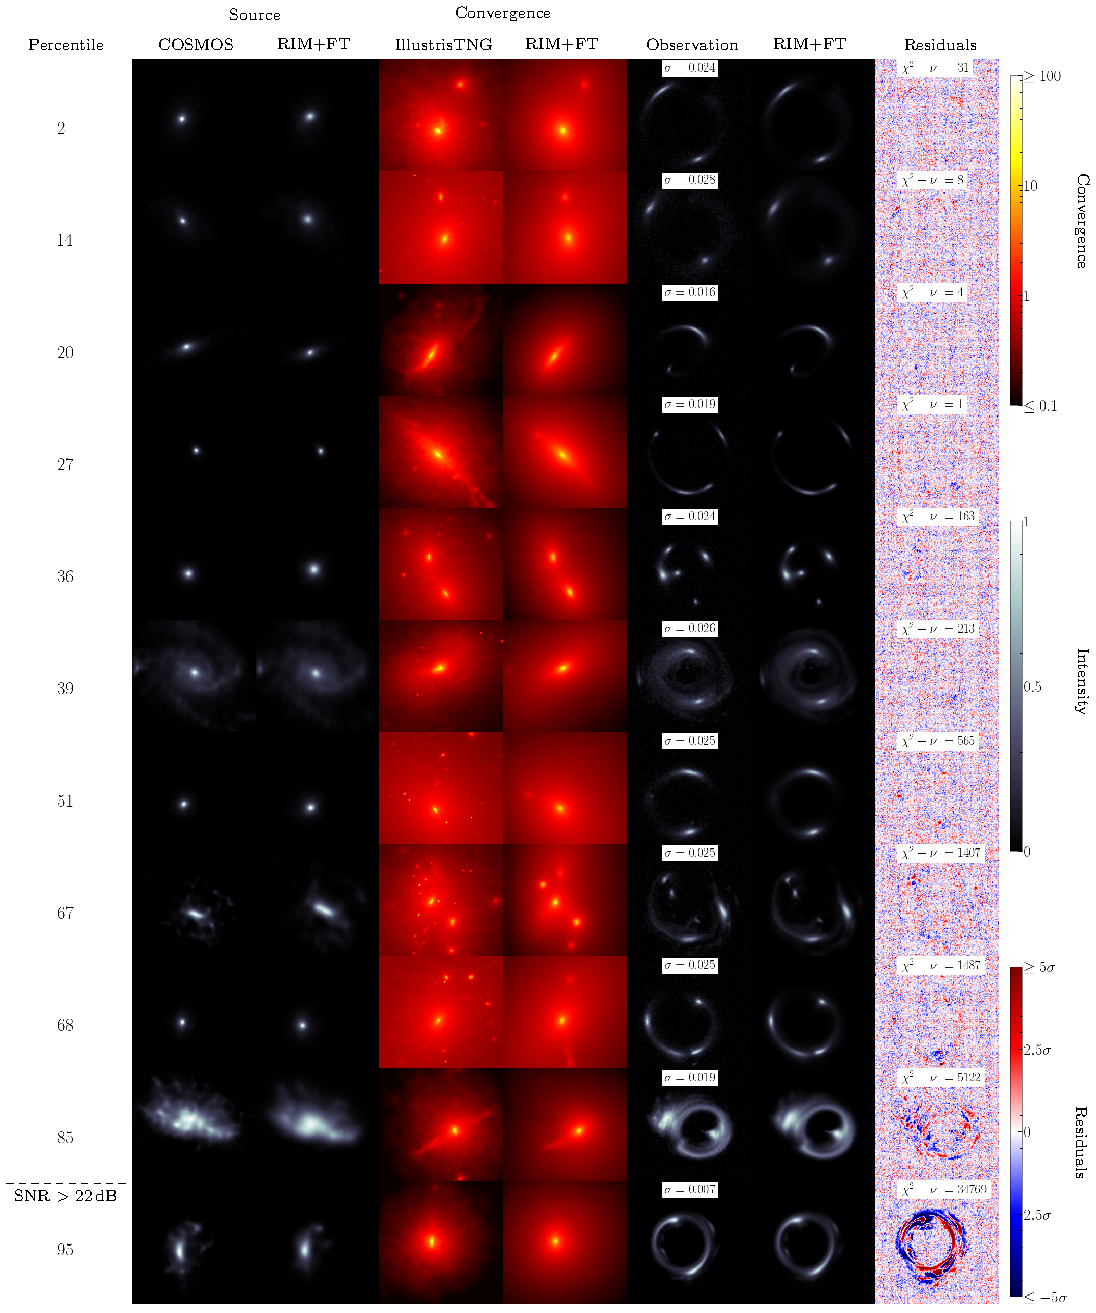
\includegraphics[width=0.90\linewidth]{figures/main_result}
        \caption{
                Cherry-picked sample of the fine-tuned RIM reconstructions 
                on a test set of 3000 examples. 
                Examples are ordered from the best $\chi^2$ (top) to the worst (bottom). 
                The percentile rank of each example is in the leftmost column. 
                The last example 
        shown has SNR above the threshold defined in Figure \ref{fig:chi squared vs noise}.}
        \label{fig:main result}
        \vspace{-1.5pt} % fix
\end{figure}

\begin{figure}[H]
        \centering
        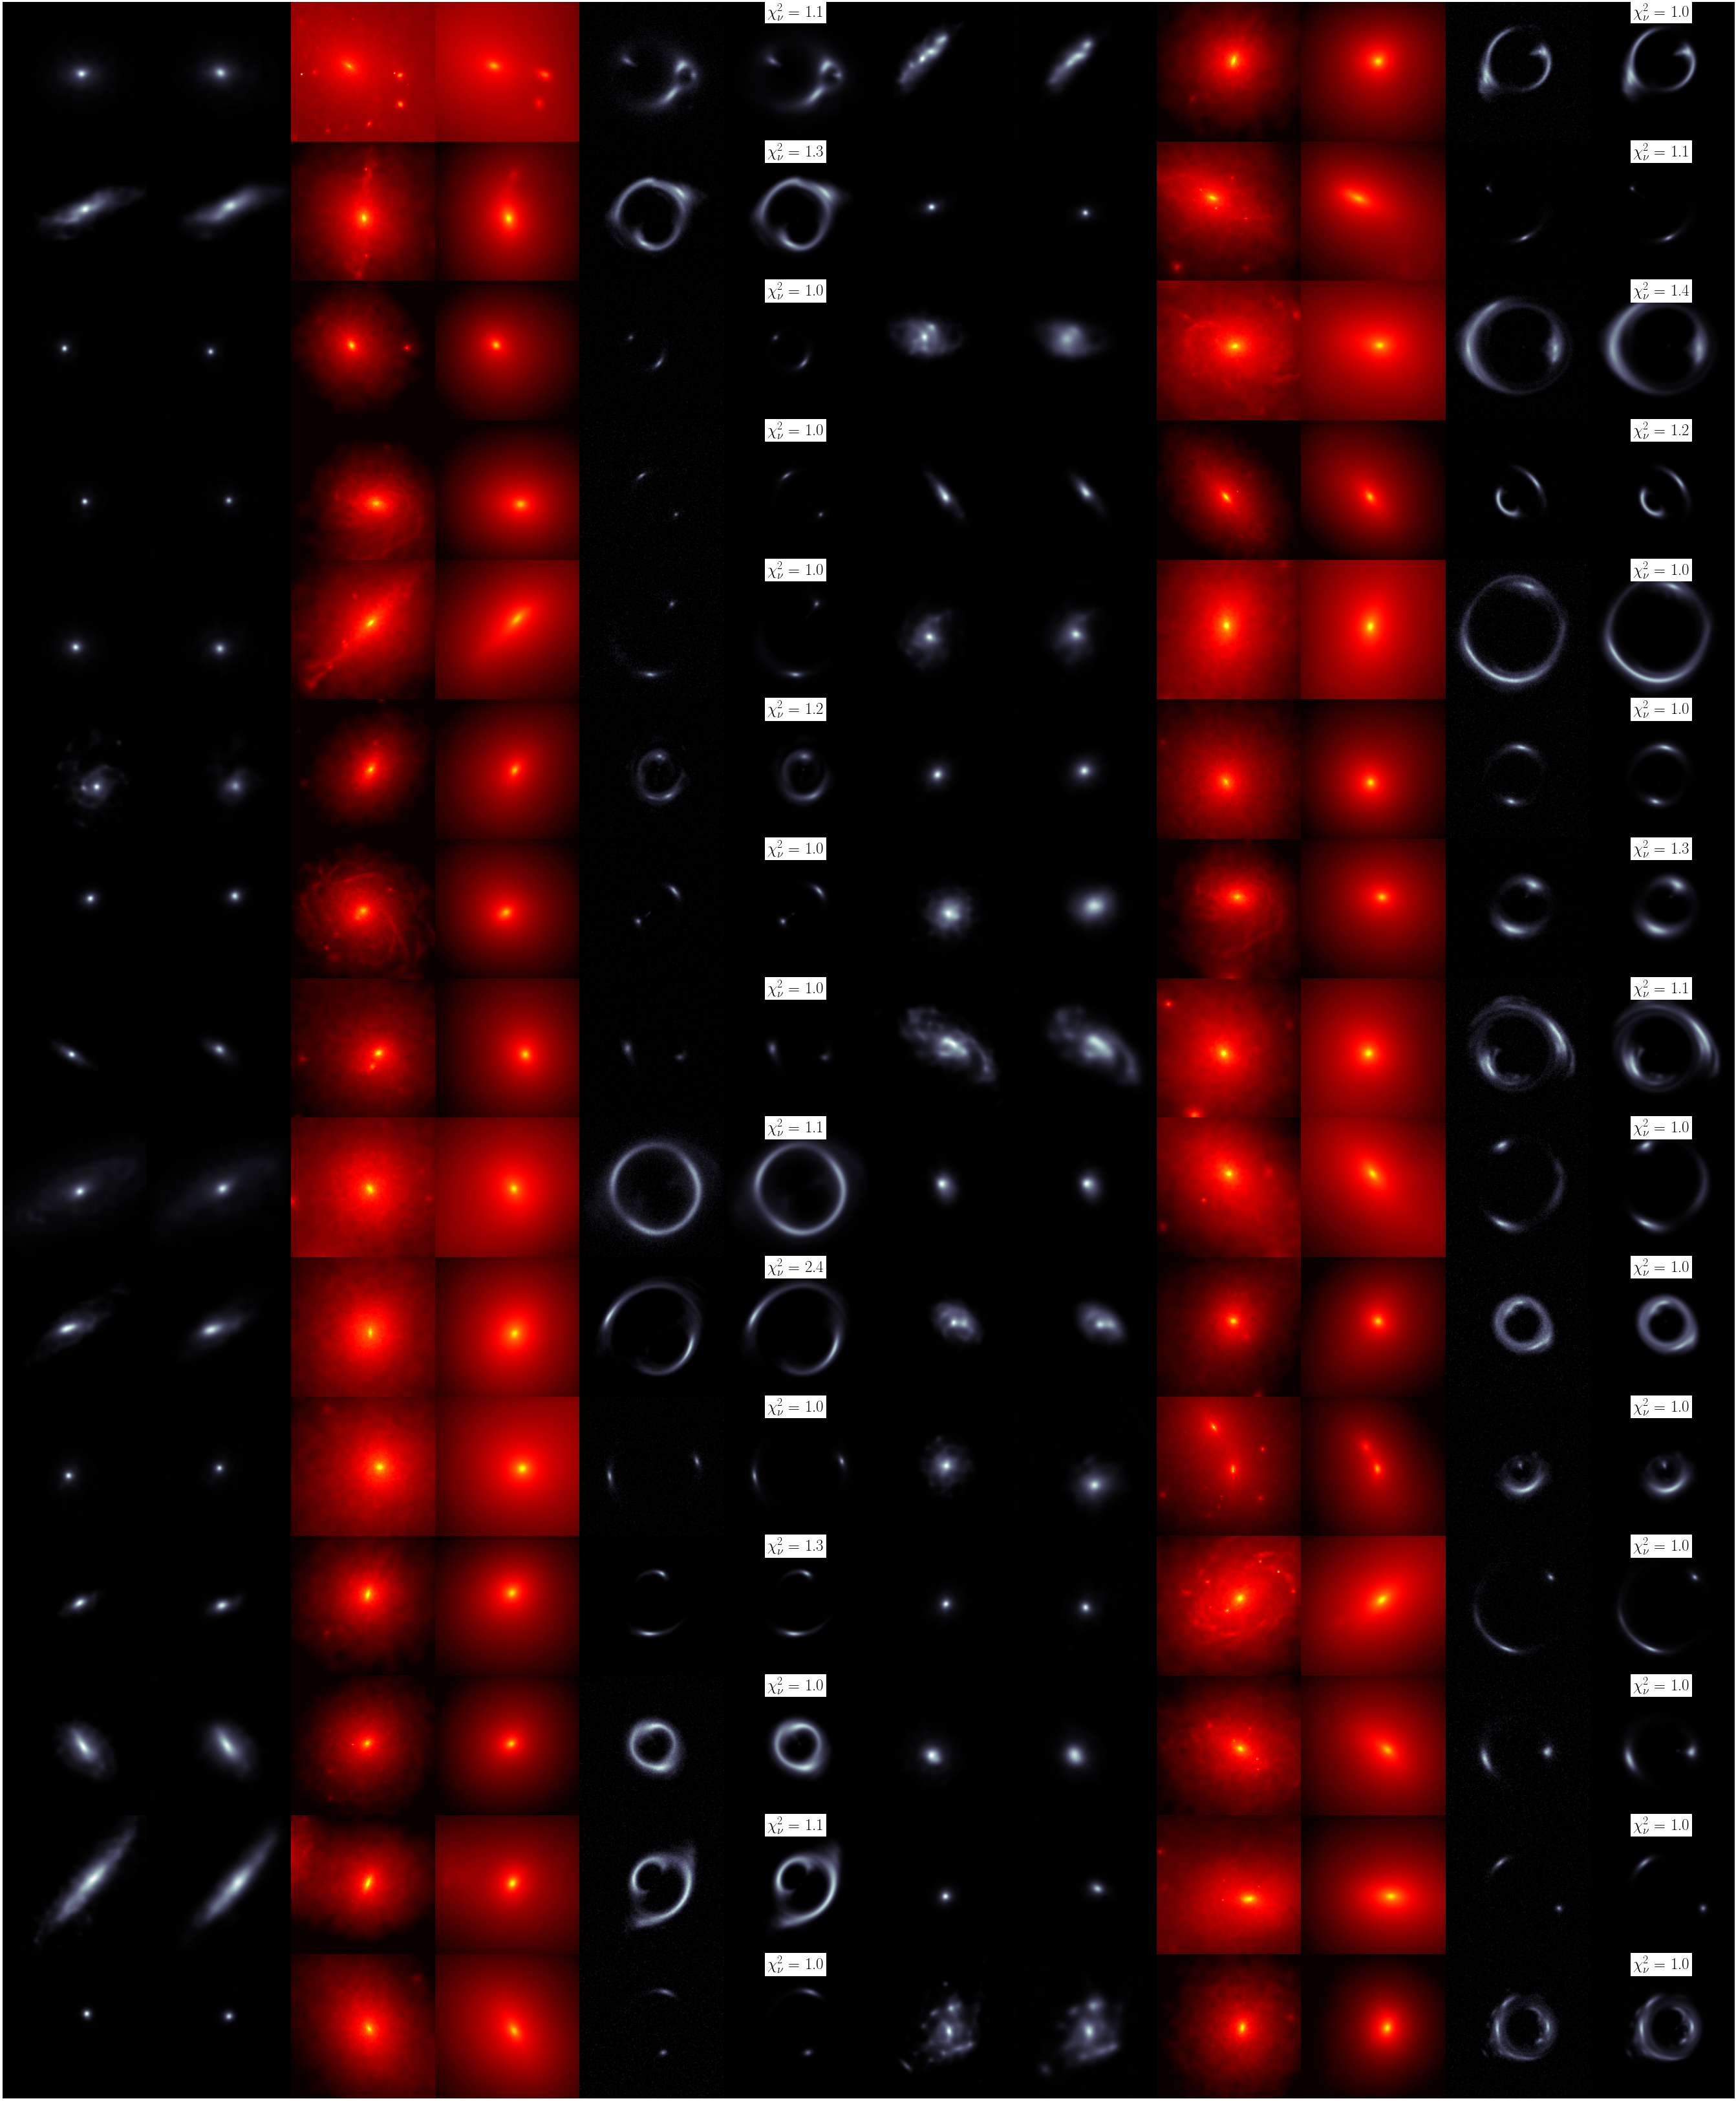
\includegraphics[width=\linewidth]{figures/test_set_no_cherry_pick}
        \caption{
                30 reconstructions taken at random from the test set of 3000 examples simulated from COSMOS 
                and IllustrisTNG data at high SNR.
                The colorscale are the same as in Figure \ref{fig:main result}.}
        \label{fig:random sample}
\end{figure}

\begin{figure}[H]
        \centering
        \tikzset{font={\fontsize{8pt}{12}\selectfont}}
        \begin{tikzpicture}
                \node at (0, 0) {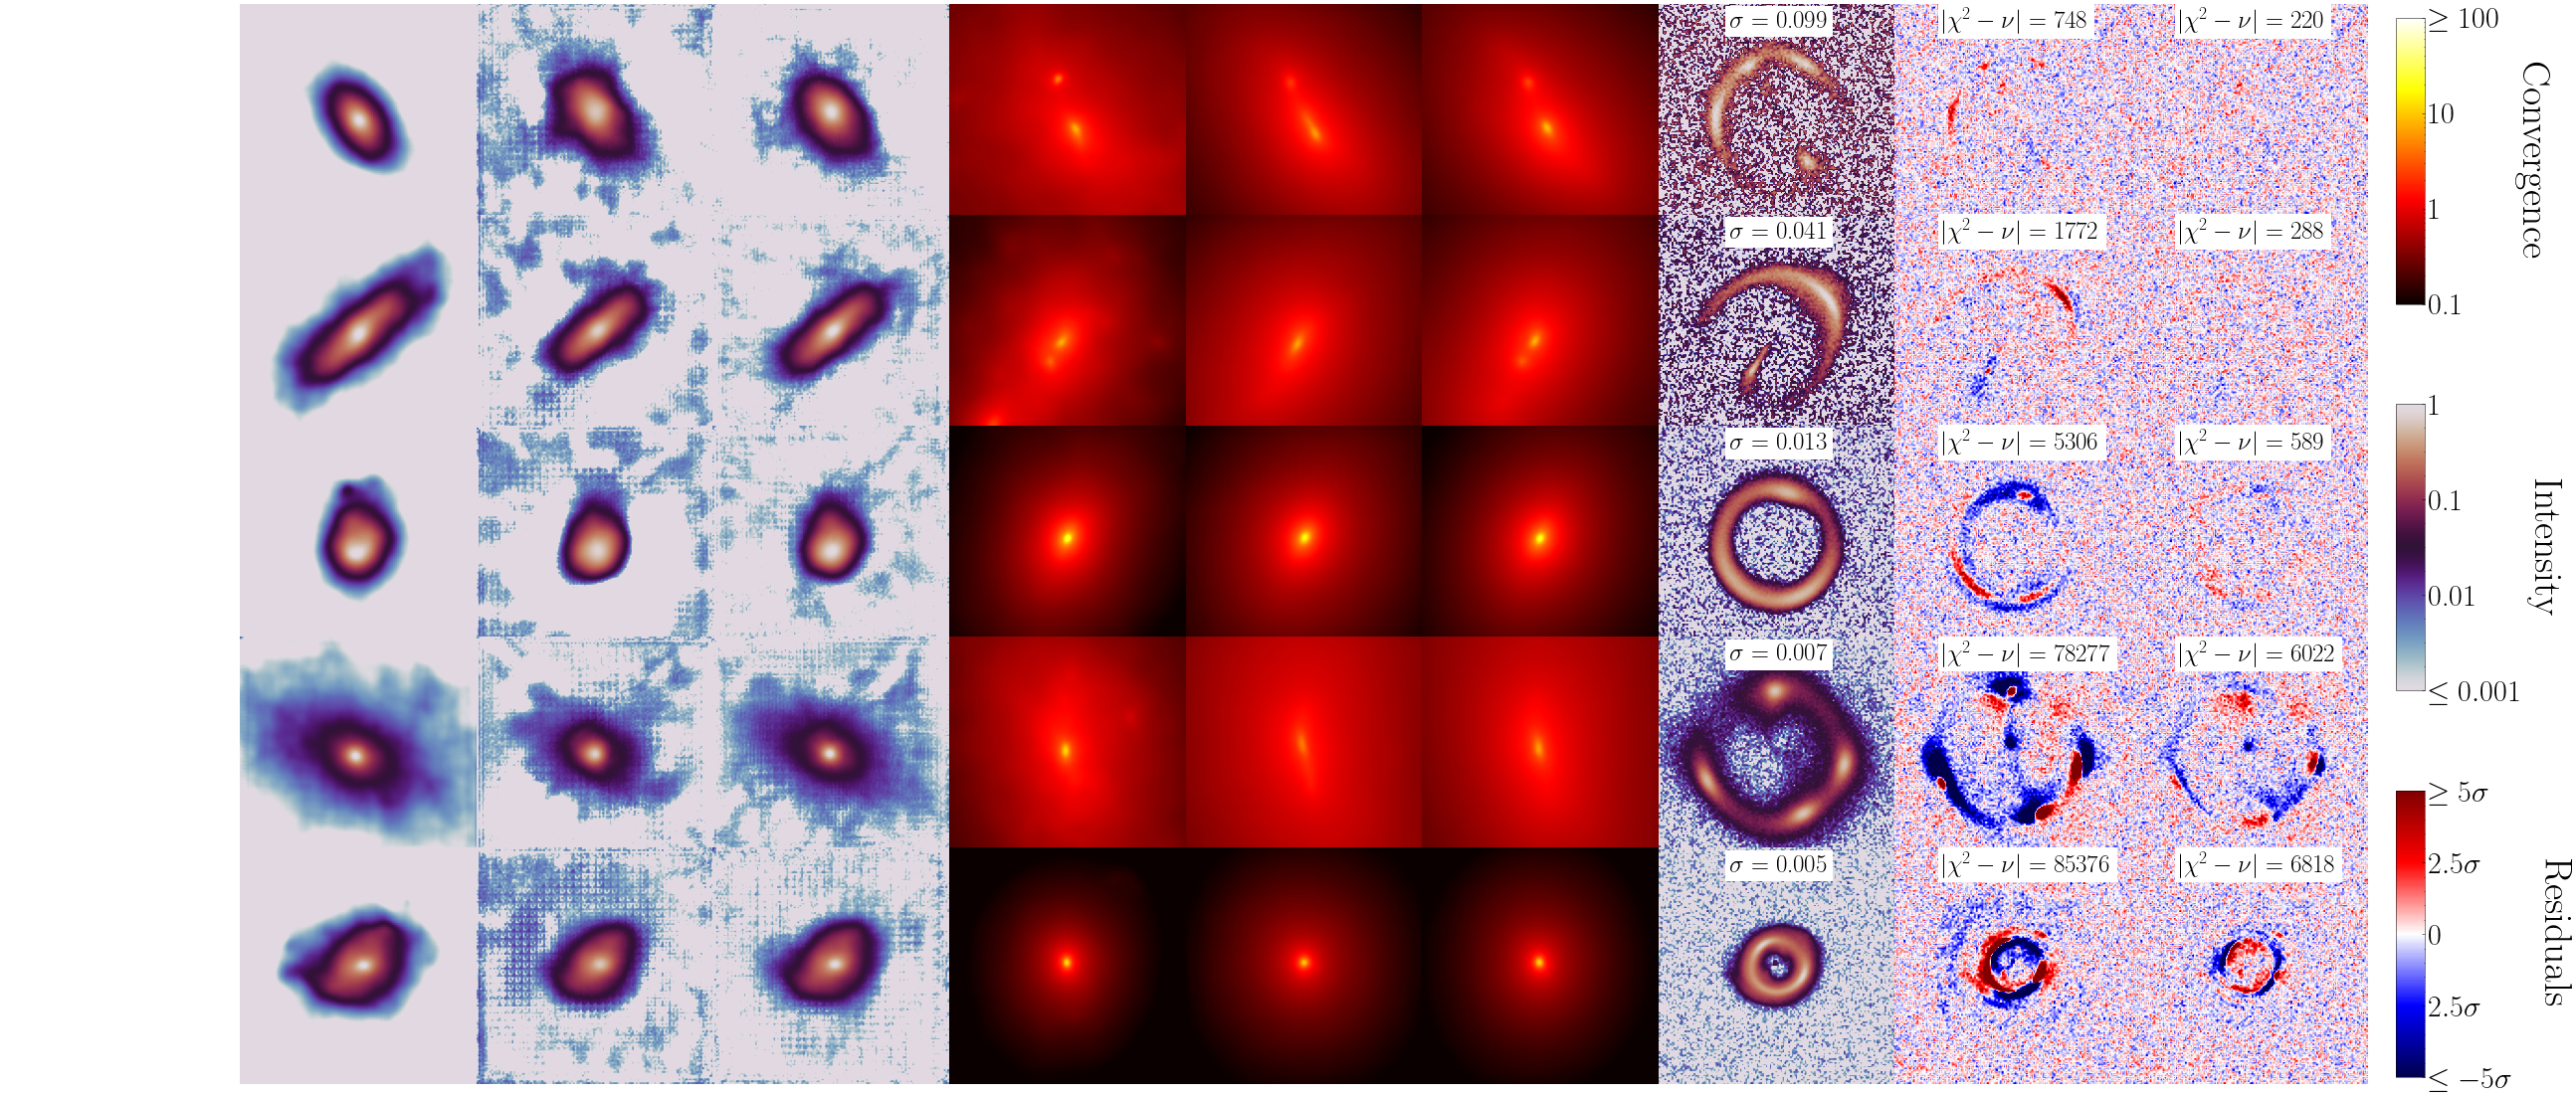
\includegraphics[width=\linewidth]{figures/rim_map_on_vae_cherry_picks}};
                \draw[-latex] (-7, 3.2) -- (-7, -3.2) node[midway, above, rotate=90] {Increasing SNR};
                %\node at (-6, 4.3) {\strut GT};
                \node at (-3.8, 4.2) {\strut Reconstruction};
                \node at (-6, 3.7) {\strut VAE};
                \node at (-4.5, 3.7) {\strut RIM};
                \node at (-3 , 3.7) {\strut RIM+FT};
                %\node at (-1.5, 4.3) {GT};
                \node at (0.9, 4.2) {\strut Reconstruction};
                \node at (-1.5, 3.7) {\strut VAE};
                \node at (0.1, 3.7) {\strut RIM};
                \node at (1.6, 3.7) {\strut RIM+FT};
                \node at (3.2, 3.7) {\strut Observation};
                \node at (5.5, 4.2) {\strut Residuals};
                \node at (4.6, 3.7) {\strut RIM};
                \node at (6.1, 3.7) {\strut RIM+FT};
        \end{tikzpicture}
        \caption{
        Comparison between baseline (RIM) and fine-tuned (RIM+FT) reconstructions for VAE generated 
        gravitational lensing systems. 
        From top to bottom, we increase SNR. The first 2 
        rows have noise level reconstruction, while the last 3 row show significant improvement 
        over the baseline. The intensity color scale is chosen to show the reconstruction
down to the third decimal place, where the baseline prediction breaks down.}
        \label{fig:increasing SNR}
\end{figure}



To understand why some of the reconstructions do not reach noise level, we 
report the joint distribution of the reduced chi squared and the SNR in Figure \ref{fig:chi squared vs noise}.
Two behaviors can be identified. For SNR below a certain threshold, the goodness of fit 
of the fine-tuned model is essentially flat, with a certain scatter, around the noise level. 
This scatter increases as a function of SNR, which reflects the fact that high-SNR reconstructions are much more difficult to perform than low-SNR observations (for any model or algorithm, not just ours) because they require very precise assumptions about the solution. 
Near the threshold, this scatter is at its peak. This is SNR regime ($18\,\mathrm{dB} \lesssim \mathrm{SNR} \leq 22\,\mathrm{dB}$) is where most of the fine-tuned reconstructions which do not reach noise level are found ($|\chi^2 - \nu| > 296$).
For SNR above the threshold, 
the goodness of fit follows the trend $\chi^2 \propto \sigma^{-2}$, which 
means the reconstructions have stopped improving on par with the noise level.
We define an optimistic threshold at the data point with largest 
SNR value which still have statistically significant residuals ($|\chi^2 - \nu| < 296)$. We 
find this threshold value to be $22\, \mathrm{dB}$ based on the test set. 

%We can interpret this result in light of the data processing inequality \citep[DPI,][]{Cover2006}. 
%We might view this in the context of three random variable in a Markov chain $X \rightarrow Y \rightarrow \hat{X}^{(T)}$ 
%where $Y$ is be the observed lensed image, $\hat{X}^{(T)}$ is the compressed statistics
%predicted by the RIM and $X$ is the original 
%model parameters (source and convergence). DPI then states that no function of $Y$, e.g. $G_\varphi(Y) = \hat{X}^{(T)}$, 
%can increase the amount of information of $Y$ about $X$. 
%In term of the mutual information of the random 
%variables, we write
%\begin{equation}\label{eq:DPI}
        %I(X; Y) \geq I(X; \hat{X}^{(T)})
%\end{equation} 
%We note that a U-net does not behave as a Markov chain unlike single-stream deep neural networks 
%\citep{Tishby2015,Tapia2020} because of the 
%skip connections as was observed by \citet{Lee2021}. Although we placed GRUs inside 
%these skip connection, we argue that the recurrent relation \ref{eq:RIM} essentially 
%act as a skip connection, thus the inequality only hold in a global sense and not between 
%different states $X^{(t)}$. On the contrary, we would expect $I(X ; \hat{X}^{(t)})$ to increase 
%as a function of $t$. 


To understand this threshold behavior, 
we inspected some source reconstructions with intensity plotted in log scale 
in Figure \ref{fig:increasing SNR}. As can seen in this figure, the source pixel intensities of the 
RIM prediction in the regime $\mathrm{SNR} \gtrsim 22\,\mathrm{dB}$, meaning the third decimal place of the reconstructed 
intensity values shown in pale blue, do not have a coherent structure and 
correspond mostly to numerical errors, even for the fine-tuned network. Reducing the noise 
level in the observed lensed image does not change this behavior, which indicates that this is a limitation 
of the neural network itself. Thus, we argue that the threshold can be explained in part because 
the inductive biases learned by the neural network during training prohibits the fine-tuning 
procedure to reconstruct the signal past the threshold value via the EWC prior term. Reducing the 
strength of the prior will not improve the reconstruction since fine-tuning with
$\lambda \ll 2\times 10^5$ will quickly produce noise leakage in the source reconstruction.

Since the threshold value found is large enough to apply our method to most known 
gravitational lens images \citep{Bolton2008,Shu2017},
we leave further investigations to future works.
We note that we purposefully ignored the 
low SNR regime since analytical methods perform well in that regime --- at low SNR, simple 
Sersic \citep{Sersic1963} and SIE \citep[]{keeton2001} models will often give good fit to the data 
since most of the information about the source and the convergence morphology is lost.
%We note that a RIM also performs well in the low SNR regime, unlike feed-forward neural networks, because 
%of the recurrent relation \eqref{eq:RIM}. Our test suggested that our model can perform 
%meaningful reconstructions up to $\sigma \lesssim 0.2$ for some of our systems. 
%Furthermore,
%our tests of the RIM suggested that it can perform meaningful reconstructions up to $\sigma \lesssim 0.2$.
%making our approach well suited for most known HST gravitational lens images 




%\vfill\null 

\subsection{Quality of the Reconstructions}\label{sec:quality of reconstructions}

\begin{figure}[th!]
        \centering
        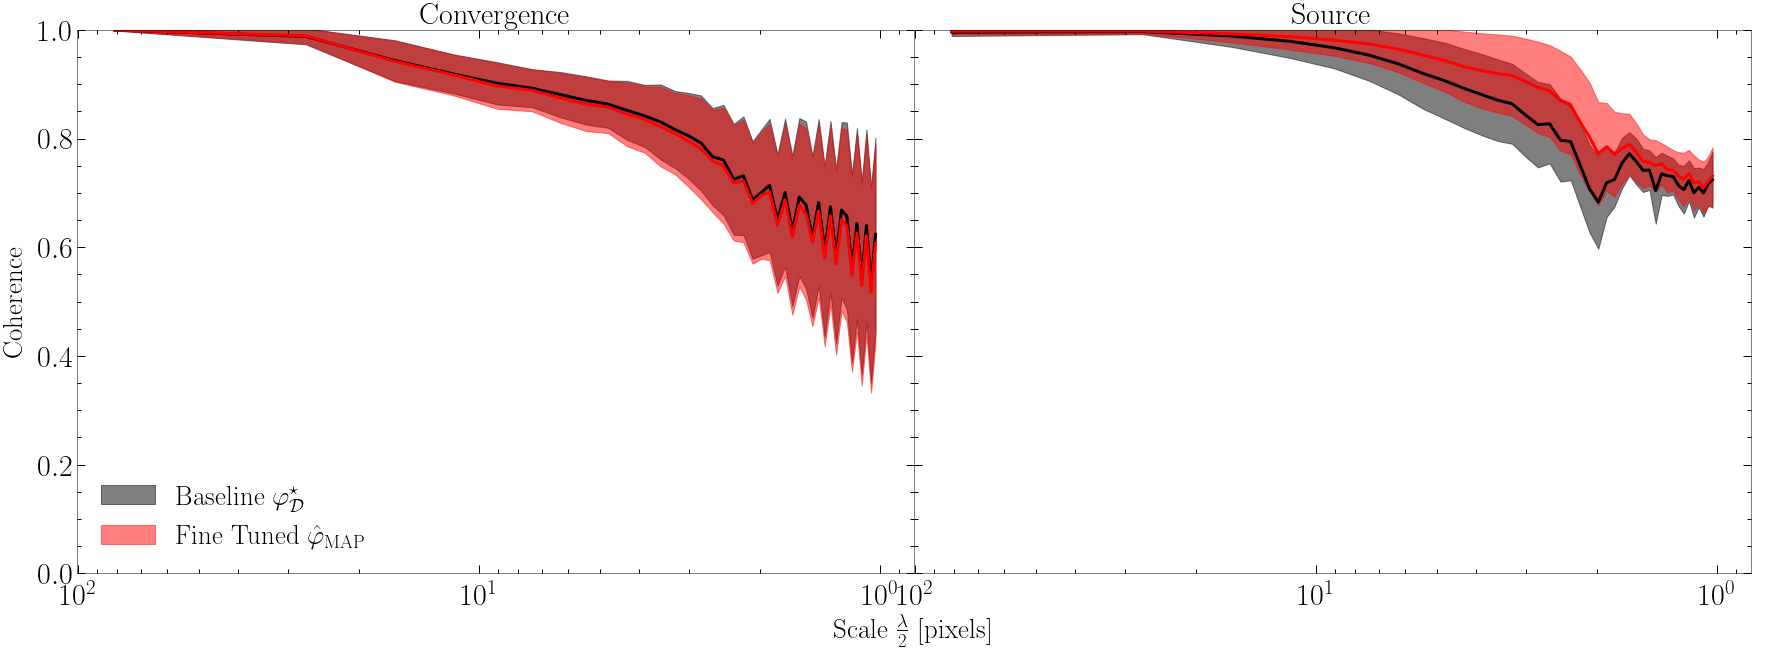
\includegraphics[width=0.7\linewidth]{figures/coherence_spectrum}
        \caption{Statistics of the coherence spectrum on the test set. The solid line is the average 
        coherence. The transparent region is the $68\%$ confidence interval. The fine-tuning 
        procedure yields a noticeable improvement on the coherence of the source at all frequencies.}
        \label{fig:coherence}
\end{figure}


In addition to a visual inspection of the reconstructed sources 
and convergences, we compute 
the coherence spectrum to quantitatively assess the quality of the reconstructions
\begin{equation}\label{eq:coherence} 
        \gamma(k) = \frac{P_{12}(k)}{\sqrt{P_{11}(k) P_{22}(k)}} \, .
\end{equation}
$P_{ij}(k)$ is the cross power spectrum of images $i$ and $j$ at 
the wavenumber $k$. Figure \ref{fig:coherence} shows the mean value and the $68\%$ inclusion interval of $\gamma(k)$ 
for the convergence and source maps in a test set of 3000 examples. 
The fine-tuning 
procedure, shown in red, is able to improve significantly the coherence of the baseline background 
source, shown in black, at all scales. 
The coherence spectrum of the convergence remains unchanged by the fine-tuning procedure.
Still, we note that many examples in the dataset showcase significant 
improvement which we illustrate in Figure \ref{fig:main figure}.
%In this case, the observed lensed image exhibits a large deflection in 
%its eastern arc which indicates the presence of a massive object --- in this 
%case a dark matter subhalo. The fine-tuning procedure is able to recover 
%this subhalo because of its strong signal in the lensed image.


%\begin{figure}[h!]
        %\centering
%\begin{tikzpicture}[every node/.style={inner sep=0,outer sep=0}]
        %\node at (-2, 1.2) {Baseline};
        %\node at (-2, 0) {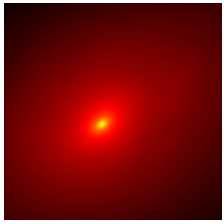
\includegraphics[width=2cm]{figures/kappa_baseline_1396}};
        %\node at (0, 1.2) {Fine-tuned};
        %\node at (0, 0) {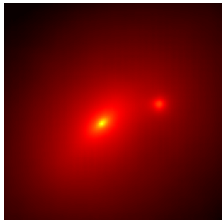
\includegraphics[width=2cm]{figures/kappa_ft_1396}};
        %\node at (2, 1.2) {Ground Truth};
        %\node at (2, 0) {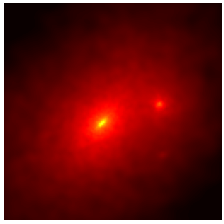
\includegraphics[width=2cm]{figures/kappa_1396}};
        %\node at (4, 1.2) {Observation};
        %\node at (4, 0) {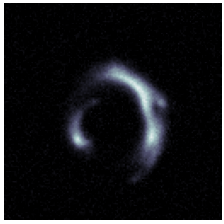
\includegraphics[width=2cm]{figures/obs_1396}};
%\end{tikzpicture} 
%\caption{Comparison between a baseline and fine-tuned reconstruction of a 
%convergence map.}
%\label{fig:convergence}
%\end{figure}


\section{Conclusion}\label{sec:conclusion}
%In this work, we introduced a framework for free-form gravitational 
%lensing inference at high SNR. This is an improvement upon traditional modeling. 
%Our framework can recover MAP point estimate of both the source and the convergence on pixelated grids 
%with high precision and high accuracy, for a wide range of gravitational lensing configurations.

%We believe that this framework will enable detailed modelling of present high SNR data and 
%upcoming images from facilities like the James Webb Telescope, thereby pushing our understanding of 
%dark matter and baryonic matter distribution at the very small scale.

The results obtained here demonstrate the effectiveness of machine learning methods for inferring pixelated maps of the distribution of mass in lensing galaxies. Since this is a heavily under-constrained problem, stringent priors are needed to avoid overfitting the data, a task that has traditionally been difficult to accomplish \citep[e.g.,][]{Saha1997}. The model proposed here can implicitly learn these priors from a set of training data. 

The flexible and expressive form of the reconstructions means that, in principle, any lensing system (e.g., a single simple galaxy, or a group of complex galaxies) could be analyzed by this model, without any need for pre-determining the model parameterization. This is of high value given the diversity of observed lensing systems, and their relevance for constraining astrophysical and cosmological parameters. 

Another significant advantage of the proposed method is that the true physical model (a ray-tracing simulation code here) is used at every iteration to calculate the likelihood of the RIM predictions given the observations, which significantly helps with the interpretability of the model and the obtained results. 

Finally, perhaps the most important limitation of the method is the fact that, in its current form, the model only provides point estimates of the parameters of interest. Quantifying the posteriors of such high-dimensional data may require a generative process. In future work, we will explore the possibility of sampling from latent variables within the RIM to obtain samples from the posteriors.  

\section*{Software and data}
The source code, as well as the various scripts and parameters used to 
produce the model and results is available as open-source software 
under the package \texttt{Censai}\footnote{
\href{https://github.com/AlexandreAdam/Censai}{

\includegraphics[scale=0.25]{figures/GitHub-Mark-32px.png}
https://github.com/AlexandreAdam/Censai}}. 
The model parameters, as well as convergence maps used to train 
these models and the test set examples and reconstructions results are also available as open-source datasets hosted by Zenodo\footnote{\href{https://doi.org/10.5281/zenodo.6555463}
{
\includegraphics[scale=0.1]{figures/zenodo}
https://doi.org/10.5281/zenodo.6555463}}. This research made use of \texttt{Tensorflow} \citep{tensorflow}, 
\texttt{Tensorflow-Probability} \citep{tensorflow-probability}, 
\texttt{Numpy} \citep{numpy}, 
\texttt{Scipy} \citep{scipy}, 
\texttt{Matplotlib} \citep{matplotlib}, 
\texttt{Scikit-image} \citep{scikit-image}, 
\texttt{IPython} \citep{ipython}, 
\texttt{Pandas} \citep{pandas1,pandas2}, 
\texttt{Scikit-learn} \citep{scikit-learn}, 
\texttt{Astropy} \citep{astropy:2013,astropy:2018} 
and \texttt{GalSim} \citep{galsim}.

%\section*{Acknowledgements}
%We thank Ronan Legin for fruitful discussion and insights about 
%training the neural network and comments about the manuscript.
%This research was supported by the Schmidt Futures Foundation. The work was also enabled in part by computational resources provided by Calcul Quebec, Compute Canada and the Digital Research Alliance of Canada. Y.H. and L.P. acknowledge support from the National Sciences and Engineering Council of Canada grant RGPIN-2020-05102, the Fonds de recherche du Québec grant 2022-NC-301305, and the Canada Research Chairs Program. A.A. was supported by an IVADO scholarship.
%\clearpage
%\bibliography{bibliography}
%\appendix

%\section{Variational Autoencoder (VAE)}\label{ap:VAE}
%When working with limited data, data augmentation is crucial to insure that 
%the trained model is robust against all sort of perturbations ---
%like rotations of an image --- that are not directly included as symmetries in the 
%architecture of the model. In that sense, data augmentation is a way to 
%induce (or remove) 
%a bias via \ref{prior:data} that is not enforced by \ref{prior:architecture}.
%In section 
%\ref{sec:dataset}, we discuss the different methods for 
%augmentations applied to our data. 
%In this section, we discuss a generative modelling approach 
%to data augmentation that will complement the other ones.

%VAEs were originally introduced by \citet{Kingma2013} as a framework to do approximate inference on 
%intractable posterior distributions with a latent variable graphical model. 
%We aim here to briefly 
%cover the most salient concepts related to our work, and refer
%the reader to the white paper of \citet{Kingma2019}.

%A VAE is decomposed into two parts. On the one hand, an encoder 
%$q_\phi$ is a stochastic function which approximate the 
%posterior of a latent variable $\mathbf{z}$:
%\begin{equation}\label{eq:VAE}
%q_{\phi} (\mathbf{z} \mid \mathbf{x}) \approx p_{\theta}(\mathbf{z} \mid \mathbf{x}).
%\end{equation} 
%On the other hand, the decoder networks with parameters $\theta$ 
%is the generative part of the VAE. It learns to decode 
%the latent space into meaningful features of the data $\mathbf{x}$. 
%In this sense, the generative model goal is to learn a posterior 
%of the data $p_{\theta}(\mathbf{x} \mid \mathbf{z})$.
%The objective function for this problem 
%is the evidence lower bound {($\mathcal{L}_{\phi,\theta}$: ELBO)} 
%which aims to satisfy \eqref{eq:VAE}:
%\begin{equation}\label{eq:ELBOth}
%\mathcal{L}_{\phi,\theta}(\mathbf{x}) =
        %\EX_{q_\phi} \big[\log p_{\theta}(\mathbf{x}) \big]
        %- D_{\mathrm{KL}}\big(q_\phi(\mathbf{z} \mid \mathbf{x}) \Vert p_\theta (\mathbf{z} \mid \mathbf{x}) \big).
%\end{equation} 
%To make this problem tractable, we assume the latent 
%variable distributions should follow a normal 
%distribution with a diagonal covariance matrix: 
%\begin{equation}\label{eq:Latent}
        %p(\mathbf{z}) \sim \mathcal{N}(0, \bbone)
%\end{equation} 
%Under the reparameterization trick \citep{Kingma2013}
%\begin{equation}\label{eq:Reparametrization}
%\begin{aligned}
        %\boldsymbol{ \epsilon} &\sim \mathcal{N}(0, \bbone)\\
        %(\boldsymbol{\mu}, \log \boldsymbol{\sigma}) &= \mathrm{Encoder}_{\phi}(\mathbf{x})\\
        %\mathbf{z} &= \boldsymbol{ \mu} + \boldsymbol{ \sigma} \odot \boldsymbol{ \epsilon},
%\end{aligned} 
%\end{equation} 
%the ELBO 
%can then be differentiated w.r.t $\phi$ and $\theta$ since this choice 
%yields a tractable ELBO with a functional form 
%described by equation (10) of \citet{Kingma2013}:
%\begin{equation}\label{eq:ELBO} 
        %\mathcal{L}_{\phi,\theta} \simeq 
        %\log p_{\theta}(\mathbf{x} \mid \mathbf{z})
        %+
        %\frac{\beta}{2}\sum_{j=1}^{J} \big( 1 + \log(\boldsymbol{\sigma}_j^{2}) - \boldsymbol{\mu}_j^{2} - \boldsymbol{\sigma}_j^{2}\big).
%\end{equation} 
%We've introduced the $\beta$ parameters to balance the KL term with the 
%reconstruction error as mentionned in section \ref{sec:vae training}.
%Once trained, the generative model $\mathrm{Decoder}_\phi (\mathbf{z})$ 
%can be used to generate new examples from the latent space $\mathbf{z} \sim \mathcal{N}(0, \bbone)$.



%\section{Sampling similar lensing systems}\label{ap:AE}



%\section{Elastic Weight Consolidation}\label{ap:ewc}

%Suppose we are given a training set $\mathcal{D}$ and a test task $\mathcal{T}$. The 
%posterior of the RIM parameters $\mathcal{\varphi}$ can be rewritten using the Bayes rule as
%\begin{equation}
        %p(\varphi \mid \mathcal{D},\, \mathcal{T}) = 
        %\frac{p(\mathcal{T} \mid \mathcal{D},\, \varphi) p(\varphi \mid \mathcal{D})}
        %{p(\mathcal{T} \mid \mathcal{D})}.
%\end{equation} 
%We suppose that $\varphi$ encode 
%information about $\mathcal{D}$, while $\mathcal{T}$ was unseen by $\varphi$. 
%It follows that 
%$\mathcal{T}$ and $\mathcal{D}$ are conditionally independent when given $\varphi$. 
%We do not make the stronger assumption that $\mathcal{D}$ and $\mathcal{T}$ 
%are completely independent. In fact, such an assumption 
%would contradict the premiss of our work that building a 
%dataset $\mathcal{D}$ can inform a machine (RIM) about
%task $\mathcal{T}$ --- or that, more broadly, $\mathcal{D}$ 
%contains information about $\mathcal{T}$.

%We rewrite the marginal $p(\mathcal{T} \mid \mathcal{D})$ using the Bayes rule
%in order to extract $p(\mathcal{D} \mid \mathcal{T})$, 
%the sampling distribution used to compute the Fisher diagonal elements
%\begin{equation}
        %p(\varphi \mid \mathcal{D},\, \mathcal{T}) = 
%\frac{p(\mathcal{T} \mid \varphi) p(\varphi \mid \mathcal{D})}
        %{p(\mathcal{D} \mid \mathcal{T})}
        %\frac{p(\mathcal{D})}{p(\mathcal{T})}.
%\end{equation} 
%The log-likelihood $\log p(\mathcal{T} \mid \varphi)$ is equivalent to 
%the negative of the loss function for the particular task at hand.
%In this work, we assign a uniform probability density to $p(\mathcal{T})$ and $p(\mathcal{D})$ 
%in order to ignore them.

%We now turn to the prior $p(\varphi \mid \mathcal{D})$, which 
%appears as a conditional relative to 
%the training dataset. 
%We use the Laplace approximation around the maxima $\varphi^{\star}_{\mathcal{D}}$ 
%to evaluate the prior,
%where $\varphi^{\star}_{\mathcal{D}}$ 
%are the trained parameters of the RIM that minimize the empirical risk (equation \eqref{eq:Cost}). 
%The Taylor expansion of the prior around this maxima yields
%\begin{equation}\label{app:prior}
        %\log p(\varphi \mid \mathcal{D}) \approx \log p(\varphi^{\star}_{\mathcal{D}} \mid \mathcal{D}) 
        %+ \frac{1}{2} (\varphi - \varphi^{\star}_{\mathcal{D}})^{T} 
        %\underbrace{
        %\bigg(
                %\frac{\partial^2 \log p(\varphi \mid \mathcal{D})}{\partial^2 \varphi}\bigg|_{\varphi^{\star}_{\mathcal{D}}}
        %\bigg)
%}_{\displaystyle \mathbf{H}(\varphi^{\star}_{\mathcal{D}})}
        %(\varphi - \varphi^{\star}_{\mathcal{D}}).
%\end{equation} 
%Since $\varphi^{\star}_{\mathcal{D}}$ is an extrema of the prior, the linear term vanishes. 
%The empirical estimate of the negative hessian matrix is the observed Fisher information 
%matrix which can be written as
%\begin{equation}\label{app:fisher}
        %\mathcal{I}(\varphi^{\star}_{\mathcal{D}}) = 
        %-\EX_{\mathcal{D} \mid \mathcal{T}} [\mathbf{H}(\varphi^{\star}_{\mathcal{D}})] = 
        %\EX_{\mathcal{D}\mid \mathcal{T}}
        %\Bigg[
                %\Bigg(
                %\bigg( 
                        %\frac{\partial \log p(\varphi \mid \mathcal{D})}{\partial \varphi}
                %\bigg) 
                %\bigg( 
                        %\frac{\partial \log p(\varphi \mid \mathcal{D})}{\partial \varphi}
                %\bigg)^{T}
        %\Bigg)
%\Bigg|_{\varphi^{\star}_{\mathcal{D}}}\Bigg].
%\end{equation} 
%The expectation is taken over the sample space $p(\mathcal{D} \mid \mathcal{T})$ since 
%the network parameters are held fixed during sampling.
%In order to compute the Fisher score, 
%we apply the Bayes rule to the prior to extract a loss function,
%% \begin{equation} 
%%         \log p(\varphi \mid \mathcal{D}) = \log p(\mathcal{D}\mid \varphi) 
%%         + \log p(\varphi) - \log p(\mathcal{D}).
%% \end{equation} 
%% $p(\mathcal{D} \mid \varphi)$ is the negative of a loss function, 
%which we take to be 
%proportional to the training loss (equation \eqref{eq:Loss}) and the $\chi^2$:
%\begin{equation}\label{eq:LossFisher}
        %\log p\big(\varphi \mid (\mathbf{x}, \mathbf{y}) = \mathcal{D}\big) \propto -\mathcal{L}_{\varphi}(\mathbf{x}, \mathbf{y}) + \frac{1}{T}\sum_{t=1}^{T}\log p(\mathbf{y} \mid \mathbf{\hat{x}}^{(t)}) - \frac{\ell_2}{2}\lVert \varphi \rVert^2_2
%\end{equation} 
%% The derivative of $\log p(\varphi)$ remains constant when taking 
%% the expectation in \eqref{app:fisher}.
%We find in practice the the $\ell_2$ term has little effect on the 
%Fisher diagonal and our results. Thus, we set $\ell_2 = 0$.

%Since the full Fisher matrix is intractable for a neural network, we approximate the 
%quadratic term of the prior with the diagonal of the Fisher matrix following \citet{Kirkpatrick2016}. 
%For an optimisation problem, the first term of \eqref{app:prior} is constant. Thus,
%the posterior becomes proportional to
%\begin{equation}
        %\log p(\varphi \mid \mathcal{D}, \mathcal{T}) \propto 
        %\log p(\mathcal{T} \mid \varphi ) - 
         %\frac{\lambda}{2} 
        %\sum_{j}\mathrm{diag}(\mathcal{I}(\varphi^{\star}_{\mathcal{D}}))_{j}(\varphi_j - [\varphi^{\star}_{\mathcal{D}}]_j)^2.
%\end{equation} 
%The Lagrange multiplier $\lambda$ is introduced to tune our uncertainty about the network parameters 
%during fine-tuning.

%\section{VAE Architecture and optimisation}

%For the following architectures, we employ the notion of \textit{level} 
%to mean layers in the encoder and the decoder with the same resolution. 
%In each level, we place a block of convolutional layers 
%before downsampling (encoder) or after upsampling (decoder). These operations 
%are done with strided convolutions like in the U-net architecture of the RIM.

%\begin{table}[H]
%\begin{minipage}{.5\linewidth} 
        %\centering
        %\caption{Hyperparameters for the background source VAE.}
        %\label{tab:Source VAE}
        %\begin{tabular}{cc}
                %Parameter & Value \\\hline\hline
                %Input preprocessing & $\bbone$ \\
                                    %& \\

                %\textit{Architecture} & \\
                %Levels (encoder and decoder) & 3 \\
                %Convolutional layer per level & 2 \\
                %Latent space dimension & 32\\
                %Hidden Activations & Leaky ReLU \\
                %Output Activation & Sigmoid \\
                %Filters (first level) & 16 \\
                %Filters scaling factor (per level) & 2 \\
                %Number of parameters & $3\,567\,361$\\

                           %& \\
                %\textit{Optimization} & \\
                %Optimizer & Adam \\
                %Initial learning rate & $10^{-4}$ \\
                %Learning rate schedule & Exponential Decay \\
                %Decay rate & 0.5 \\
                %Decay steps & $30\,000$ \\
                %Number of steps & $500\,000$ \\
                %$\beta_{\mathrm{max}}$ & 0.1 \\
                %Batch size & 20\\
                %\hline
        %\end{tabular}
%\end{minipage}
%\begin{minipage}{.5\linewidth}
        %\caption{Hyperparameters for the convergence VAE.}
        %\label{tab:Kappa VAE}
        %\begin{tabular}{cc}
                %Parameter & Value \\\hline\hline
                %Input preprocessing & $\log_{10}$ \\
                              %& \\

                %\textit{Architecture} & \\
                %Levels (encoder and decoder) & 4 \\
                %Convolutional layer per level & 1 \\
                %Latent space dimension & 16\\
                %Hidden Activations & Leaky ReLU \\
                %Output Activation & $\bbone$ \\
                %Filters (first level) & 16 \\
                %Filters scaling factor (per level) & 2 \\
                %Number of parameters & $1\,980\,033$\\


                           %& \\
                %\textit{Optimization} & \\
                %Optimizer & Adam\\
                %Initial learning rate & $10^{-4}$ \\
                %Learning rate schedule & Exponential Decay \\
                %Decay rate & 0.7 \\
                %Decay steps & $20\,000$ \\
                %Number of steps & $155\,000$ \\
                %$\beta_{\mathrm{max}}$ & 0.2 \\
                %Batch size & 32\\
                %\hline
        %\end{tabular}
%\end{minipage}
%\end{table}

%\section{RIM architecture and optimisation}\label{ap:rim training and opt}

%The notion of link function $\Psi: \Xi \rightarrow \mathcal{X}$, 
%introduced by \citet{Putzky2017}, is an invertible transformation 
%between the network prediction space $\boldsymbol{\xi} \in \Xi$ 
%and the forward modelling space $\mathbf{x} \in \mathcal{X}$.
%This is a different notion from preprocessing, discussed in section \ref{sec:data}, 
%because this transformation is applied inside the recurrent relation \ref{eq:RIM} 
%as opposed to before training. In the case where the forward model has some restricted 
%support or it is found that some transformation helps the training, then 
%the link function chosen must be implemented as part of the network architecture as 
%shown in the unrolled computational graph in Figure \ref{fig:unrolled graph}.
%Also, the loss $\mathcal{L}_\varphi$ must be computed in the $\Xi$ space in order 
%to avoid gradient vanishing problems when $\Psi$ is a non-linear mapping, which 
%happens if the non-linear link function is applied in an 
%operation recorded for backpropagation through time (BPTT). 


%For the convergence, we use an exponential link function with base $10$: 
%$\boldsymbol{\hat{\kappa}} = \Psi(\boldsymbol{\xi}) = 10^{\boldsymbol{\xi}}$. 
%This $\Psi$ encodes the non-negativity of the convergence. Furthermore, 
%it is a power transformation that leaves the linked 
%pixel values $\boldsymbol{\xi}_i$ normally distributed, thus improving the 
%learning through the non-linearities in the neural network.
%The pixel weights $\mathbf{w}_i$ in the loss function \eqref{eq:Loss}
%are chosen to encode the fact that the pixel with critical mass density ($\boldsymbol{\kappa}_i > 1$) 
%have a stronger effect on the lensing configuration than other pixels. 
%We find in practice that the weights 
%\begin{equation}\label{eq:convergence weights} 
        %\mathbf{w}_i = \frac{\sqrt{\boldsymbol{\kappa}_i}}{ \sum_i \boldsymbol{\kappa}_i}, 
%\end{equation} 
%encode this knowledge in the loss function and improved both the empirical 
%risk and the goodness of fit of the baseline model on early test runs.

%For the source, we found that we do not need a link function 
%--- its performance is generally better compared to other link function we tried like sigmoid and 
%power transforms --- and we found that the pixel weights can be taken to 
%be uniform, i.e. $\mathbf{w}_i = \frac{1}{M}$.


%\begin{figure}[H]
        %\centering
        %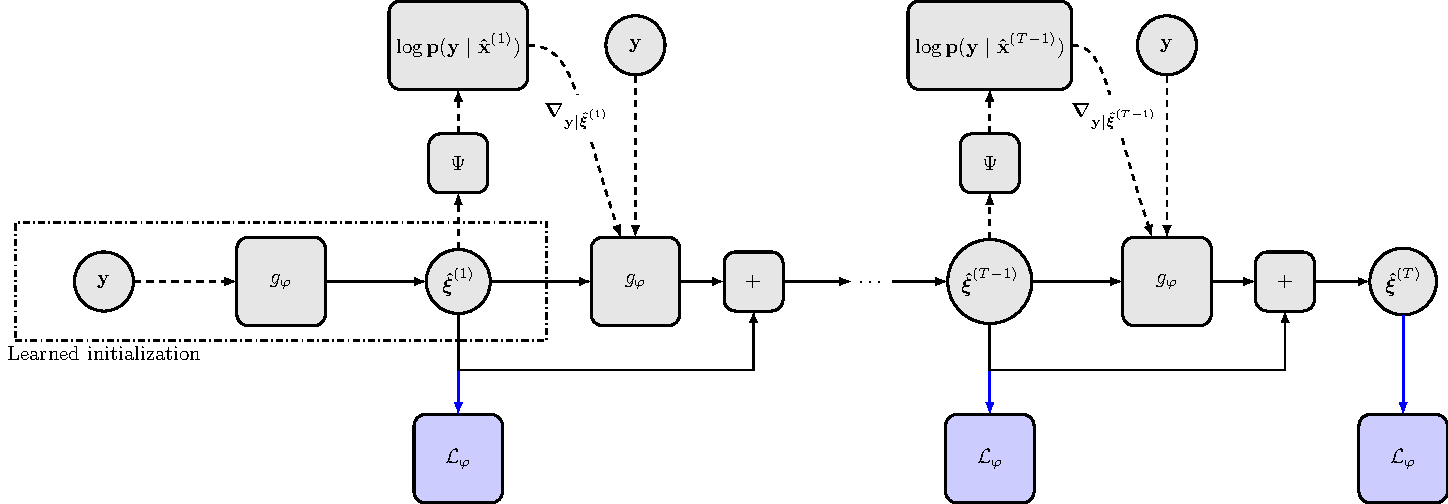
\includegraphics[width=\linewidth]{figures/schematic_rim_unrolled}
        %\caption{Unrolled computational graph of the RIM. Operations along solid arrows are being 
        %recorded for BPTT, while operations along dashed arrows are not. The blue arrows are only 
        %used for optimisation during training. During fine-tuning or testing, the loss is computed only 
        %as an oracle metric to validate that our methods can recover the ground truth.}
        %\label{fig:unrolled graph}
%\end{figure}
%\begin{table}[H]
        %\centering
        %\caption{Hyperparameters for the RIM.}
        %\label{tab:baseline hparams}
        %\begin{tabular}{cc}
                %Parameter & Value \\\hline\hline
                %Source link function & $\bbone$ \\
                %$\kappa$ link function & $10^{\boldsymbol{\xi}}$ \\
                                       %& \\
                %\textit{Architecture} & Figure \ref{fig:unet} \\
                %Recurrent steps ($T$) & 8 \\
                %Number of parameters & $348\,546\,818$ \\
                                      %& \\
                %\textit{First Stage Optimisation} & \\
                %Optimizer & Adamax \\
                %Initial learning rate & $10^{-4}$\\
                %Learning rate schedule & Exponential Decay \\
                %Decay rate & 0.95 \\
                %Decay steps & $100\,000$\\
                %Number of steps & $610\,000$\\
                %Batch size & 1 \\
                           %& \\
                %\textit{Second Stage Optimisation} & \\
                %Optimizer & Adamax \\
                %Initial learning rate & $6\times 10^{-5}$\\
                %Learning rate schedule & Exponential Decay \\
                %Decay rate & 0.9 \\
                %Decay steps & $100\,000$\\
                %Number of steps & $870\,000$\\
                %Batch size & 1 \\
                
                %\hline
        %\end{tabular}
%\end{table}





%%\section{}


%%\end{document}

